\documentclass{beamer}
\usepackage{amsmath}
\usepackage{mathtools}
\usepackage[outline]{contour}

\mode<presentation>
{
  \useoutertheme{default}
}

\beamertemplatenavigationsymbolsempty
\setbeamertemplate{frametitle}[default][center]
%\setbeamercolor{frametitle}{fg=white}
%\setbeamercolor{background canvas}{bg=black}
%\setbeamercolor{normal text}{fg=white}
%\usepackage[dvipsnames]{xcolor}
\definecolor{cyan}{rgb}{0,1,1}
\definecolor{yellow}{rgb}{1,1,0}
\definecolor{magenta}{rgb}{1,0,1}

\newcommand\DarkMode{
\setbeamercolor{frametitle}{fg=white}
\setbeamercolor{background canvas}{bg=black}
\setbeamercolor{normal text}{fg=white}
\usebeamercolor[fg]{normal text}
\setbeamercolor{item}{fg=white}
\setbeamercolor{alerted text}{fg=white}
\setbeamercolor{structure}{fg=white}
\setbeamercolor{enumerate item}{fg=white}
\setbeamercolor{author}{fg=white}
\setbeamercolor{date}{fg=white}
\setbeamercolor{institute}{fg=white}
}

\title{Network models of carcinogenesis and vestibular schwannoma}
%\subtitle{A total eclipse of the genome}
\author{Chay Paterson}
\institute{University of Manchester*}
\date{28 March 2022

\;

\tiny{*(sort of)}}
% emph. main model output: risk/incidence curve, subtype specific alterations

\begin{document}

% TODO: two graphs missing, general 3/stage multi stage
%       and evans 2005 multi-stage

\frame{\titlepage}

\begin{frame}
    \frametitle{Warning}
    \framesubtitle{There will be very few equations in this talk!}

    \begin{columns}
        \begin{column}{0.6\textwidth}
        This network...
        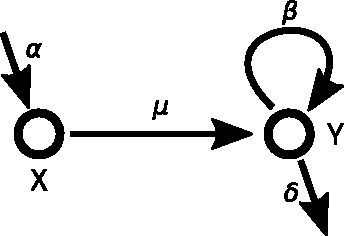
\includegraphics[width=\textwidth]{figures/diagram1}
        \end{column}
        \begin{column}{0.4\textwidth}
        corresponds to this stochastic process:...
        \begin{align}
            \emptyset \rightarrow X, &\qquad \mathrm{rate\;}\alpha
            \nonumber \\
            % NB
            X \rightarrow X + Y, &\qquad\mathrm{rate\;}\mu X
            \nonumber \\
            Y \rightarrow Y + Y, &\qquad\mathrm{rate\;} \beta Y
            \nonumber \\
            Y \rightarrow \emptyset, &\qquad\mathrm{rate\;} \delta Y
            \nonumber
        \end{align}
        \end{column}
    \end{columns}

    and approximately this linear system...

    \begin{equation*}
        \frac{d}{dt} 
        \begin{pmatrix}
            E[X] \\
            E[Y] \\
        \end{pmatrix}
        = 
        \begin{bmatrix}
            0 & 0 \\
            \mu & \beta - \delta \\
        \end{bmatrix}
        \cdot
        \begin{pmatrix}
            E[X] \\
            E[Y] \\
        \end{pmatrix}
        +
        \begin{pmatrix}
            \alpha \\
            0 \\
        \end{pmatrix}
    \end{equation*}

\begin{center}
    \small{Most of our models are linear, high-dimensional and sparse\footnotemark}
\end{center}
    % Note: example matrix
\footnotetext[1]{C. Paterson, I. Bozic, H. Clevers, PNAS 2020; 117(34): 20681-20688}
\end{frame}

% history of multi-stage models

% Replace first two slides with:
% There are many types of cancer
% with many risk factors, some unique to each (EBV?, irritants, smoking,
% alcohol)
% Three are essentially universal: age, genetics, and ionizing radiation.
% The only known risk factors for brain tumours are age, genetics, and possibly
% IR. So by learning something about these, we learn something about all
% neoplasias.

\begin{frame}
    \frametitle{What is cancer?}
    \begin{columns}
        \begin{column}{0.5\textwidth}
        % figure from Hallmarks? cliche, try something from Wellcome images
        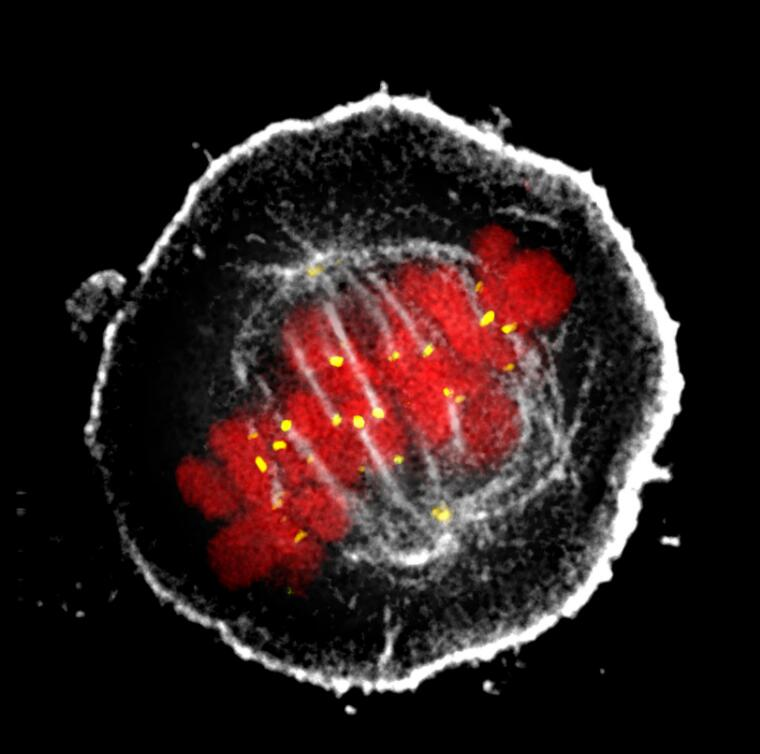
\includegraphics[width=\textwidth]{figures/HeLaCell_wellcometrust.jpg}
        \end{column}
        \begin{column}{0.5\textwidth}
            \begin{itemize}
            \item Various risk factors
            \item Mutations accumulate
            \item Loss of control of cell growth \& death
            \end{itemize}
            \begin{center}
            $\downarrow$ gets us a benign tumour/neoplasia...
            \end{center}
            \begin{center}
            $\downarrow$ something happens...
            \end{center}
            \begin{itemize}
            \item Dedifferentiation, migration...
            \item Malignancy = cancer
            \end{itemize}
        \end{column}
    \end{columns}
    \;
    \begin{center}
    \vphantom{$\sum$}
    \end{center}

\footnotetext[1]{Figure: HeLa cell https://wellcomecollection.org/works/vpgx8zcd}
\end{frame}

\begin{frame}
    \frametitle{What is cancer?}
    \begin{columns}
        \begin{column}{0.5\textwidth}
        % figure from Hallmarks? cliche, try something from Wellcome images
        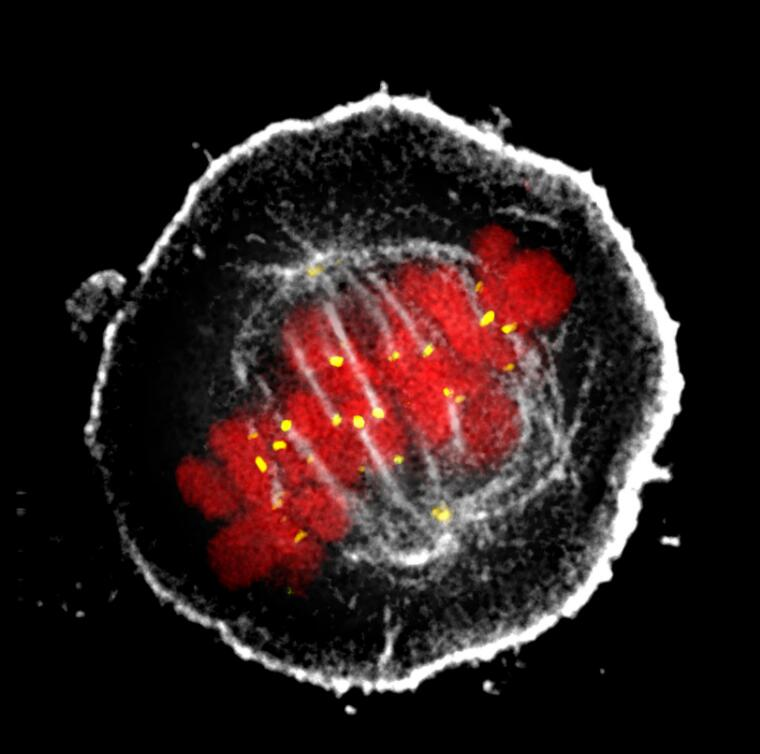
\includegraphics[width=\textwidth]{figures/HeLaCell_wellcometrust.jpg}
        \end{column}
        \begin{column}{0.5\textwidth}
            \begin{itemize}
            \item Various risk factors
            \item \underline{Mutations accumulate}
            \item Loss of control of cell growth \& death
            \end{itemize}
            \begin{center}
            $\downarrow$ gets us a benign tumour/neoplasia...
            \end{center}
            \begin{center}
            $\downarrow$ something happens...
            \end{center}
            \begin{itemize}
            \item Dedifferentiation, migration...
            \item Malignancy = cancer
            \end{itemize}
        \end{column}
    \end{columns}
    \;
    \begin{center}
    \vphantom{$\sum$}\textbf{Why do we believe this?}
    \end{center}

\footnotetext[1]{Figure: HeLa cell https://wellcomecollection.org/works/vpgx8zcd}
\end{frame}

\begin{frame}
    \frametitle{Multi-stage models}
    \framesubtitle{P. Armitage and R. Doll\footnotemark}

    % TODO add a k or N_WT to the diagram

    \begin{center}
        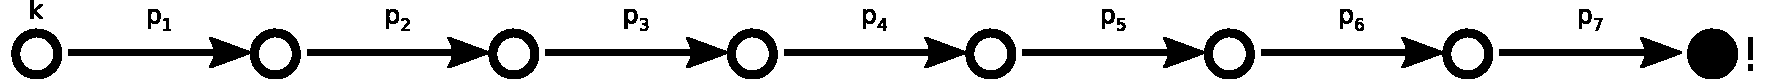
\includegraphics[width=\textwidth]{figures/diagram2b}
    \end{center}
    \begin{columns}
        \begin{column}{0.5\textwidth}
        %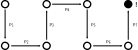
\includegraphics[width=\textwidth]{figures/diagram2}
        \begin{center}
            $\downarrow$
        \end{center}
        \begin{equation*}
            P(\mathrm{cancer}) \approx k p_1 p_2 p_3 p_4 p_5 p_6 p_7 \frac{t^7}{7!}
        \end{equation*}
        \begin{equation*}
            \implies \mathrm{incidence} \propto \frac{t^6}{6!}
        \end{equation*}
        \end{column}
        \begin{column}{0.5\textwidth}
        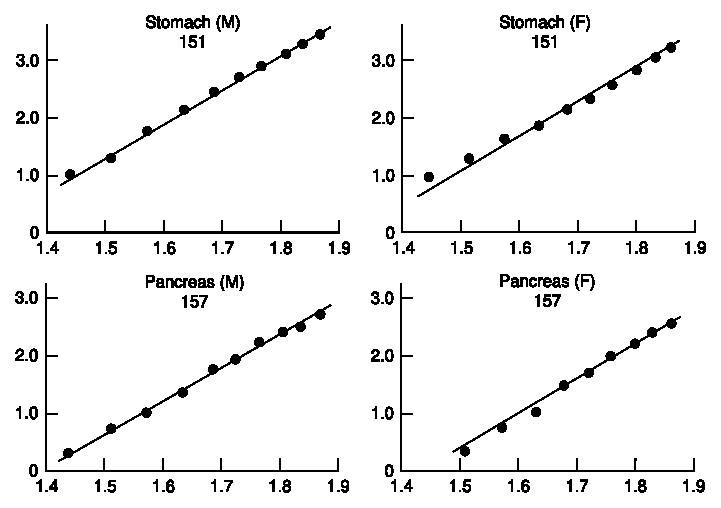
\includegraphics[width=\textwidth]{figures/PArmitageRDoll_1954_6602297.pdf}
        \end{column}
    \end{columns}

\footnotetext[1]{P. Armitage and R. Doll, British Journal of Cancer 1954; 8: 1–12}
\footnotetext[2]{note that $P(t) = 1 - S(t)$, other authors (e.g. Knudson)}
\end{frame}


% TODO slide is unnecessary: slides that are just prompts with no figures are
% boring
%\begin{frame}
%    \frametitle{Multi-stage models}
%    \framesubtitle{P. Armitage and R. Doll\footnotemark[1]}
%    \begin{center}
%    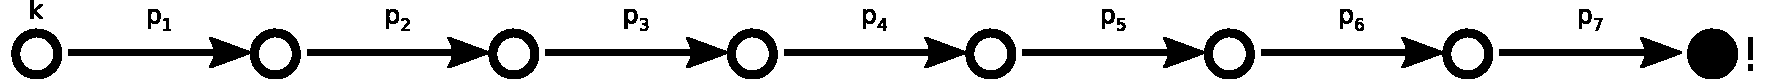
\includegraphics[width=1.00\textwidth]{figures/diagram2b}
%    \end{center}
%
%    \begin{columns}
%        \begin{column}{0.5\textwidth}
%        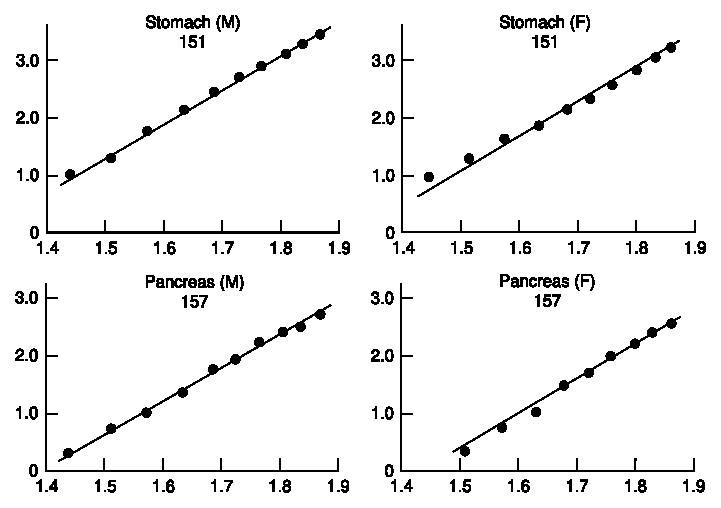
\includegraphics[width=\textwidth]{figures/PArmitageRDoll_1954_6602297.pdf}
%        \end{column}
%        \begin{column}{0.5\textwidth}
%        Problems:
%        \begin{itemize}
%            \item Parameter estimates $p_j$ implausibly high
%            \item No explicit mechanisms
%            \item Treatment of different orders of
%            events unclear \footnotemark[1]
%        \end{itemize}
%        \end{column}
%    \end{columns}
%\footnotetext[1]{P. Armitage and R. Doll, British Journal of Cancer 1954; 8: 1–12}
%\footnotetext[1]{(See Mathematical Appendix!)}
%\end{frame}

\begin{frame}
    \frametitle{Multi-stage models}
    \framesubtitle{2-3 rate limiting steps\footnotemark[123]}
    % TODO present both models
    % ie include Armitage Doll 1957 model, cite Jo Ivasa
    \begin{columns}
        \begin{column}{0.5\textwidth}
        \begin{center}
        % multi-stage clonal expansion
        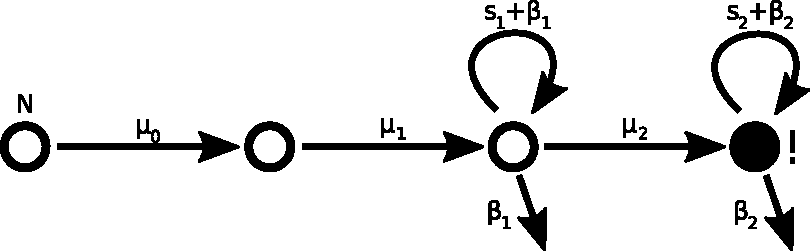
\includegraphics[width=1.00\textwidth]{figures/diagram3}
        \end{center}


        \begin{itemize}
            \item Add selection $s_k$
            \item Better fit, more plausible $\mu_k$
        \end{itemize}
        \end{column}
        \begin{column}{0.5\textwidth}
        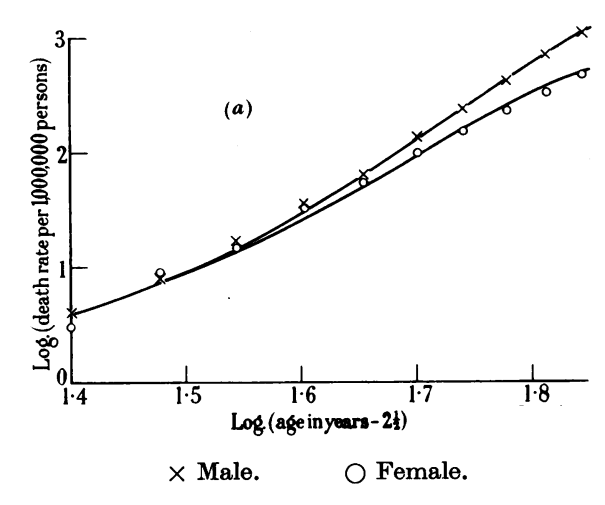
\includegraphics[width=\textwidth]{figures/ArmitageDoll1957_4A.png}
        \end{column}
    \end{columns}

    % TODO add figure from Armitage Doll 1957 etc.
\footnotetext[1]{P. Armitage and R. Doll, British Journal of Cancer 1957; 11(2): 161-169}
\footnotetext[2]{S. Moolgavkar and G. Luebeck, JNCI 1992; 84(8): 610-618}
\footnotetext[3]{F. Michor, Y. Iwasa and MA. Nowak, Nature Reviews Cancer 2004;
4: 197-205 doi:10.1038/nrc1295}
\end{frame}

% TODO replace these three slides w/a discussion of subclonal frequency
% distributions and drivers for the version at UCL:
%{
\begin{frame}
    \frametitle{Tumour suppressor genes and oncogenes}
    \begin{columns}
        \begin{column}{0.5\textwidth}
        % picture of a recessive genetic disease/predisposition
        \end{column}
        \begin{column}{0.5\textwidth}
        How are these discovered?

        \begin{itemize}
            \item Systematic searches (for something else) e.g. \emph{TP53}
            \item Linkage studies of hereditary predispositions, e.g.
            \emph{APC}, \emph{Rb}, \emph{NF2}
        \end{itemize}
        \end{column}
    \end{columns}
% interesting mathematics in pop. genetics (i.e. coalescent theory)
% check Rb linkage study claim
\end{frame}

\begin{frame}
    \frametitle{Gene prediction}
    \begin{columns}
        \begin{column}{0.5\textwidth}
        \begin{itemize}
            \item Sequencing is now very good
            \item Can predict genes by looking for ORFs and codons
        \end{itemize}
        \end{column}
        \begin{column}{0.5\textwidth}
        % Figure: sequence with start and stop codons circled in green and red
        \end{column}
    \end{columns}
\end{frame}

\begin{frame}
    \frametitle{The story so far}
    \begin{enumerate}
        \item Incidence models accurate, but agnostic re: orders and mechanisms
        \item Lots of known genes and interactions
        \item Sequencing and gene prediction advanced
    \end{enumerate}

    \begin{center}
        ...how can we systematically \emph{combine all three?}
    \end{center}
    
    \begin{center}
        \vphantom{MATHEMATICAL MODELS}
    \end{center}
\end{frame}

\begin{frame}
    \frametitle{The story so far}
    \begin{enumerate}
        \item Incidence models accurate, but agnostic re: orders and mechanisms
        \item Lots of known genes and interactions
        \item Sequencing and gene prediction advanced
    \end{enumerate}

    \begin{center}
        ...how can we systematically \emph{combine all three?}
    \end{center}
    
    \begin{center}
        \textbf{\Large{MATHEMATICAL MODELS}}
    \end{center}
\end{frame}
}


% CRC model and schwannoma
\begin{frame}
    \frametitle{Network models}
    \begin{columns}
        \begin{column}{0.5\textwidth}
        \begin{enumerate}
            \item Study \textbf{specific genes} and mechanisms of interest
            \item Fix parameters from sequences and experiments
            \item Distinguish different orders of events
        \end{enumerate}
        \begin{center}
            \textbf{Predict copy number alterations (etc.)}
        \end{center}
        \end{column}
        \begin{column}{0.5\textwidth}
        \begin{center}
            \small{example model}
        \end{center}
            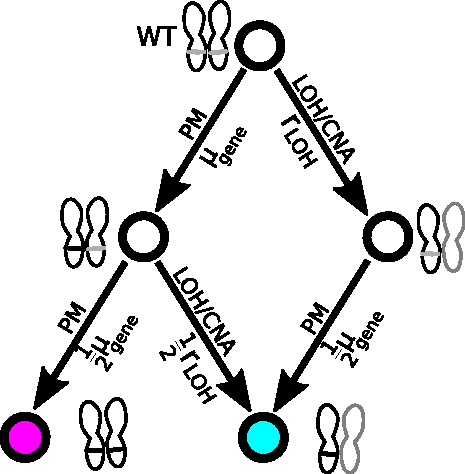
\includegraphics[width=\textwidth]{figures/diagram4}
        \end{column}
    \end{columns}

    \;

    \begin{center}
        This gets us the incidence of \emph{specific karyotypes}
    \end{center}
\end{frame}

\begin{frame}
    \frametitle{Network models}
    \framesubtitle{Worked example: tumour suppressor loss-of-function}
    % TS being lost, show how the three orders of events fold into one graph
    % emph. that one is forbidden
    \begin{center}
    Two events of interest, 3 possible orders:
    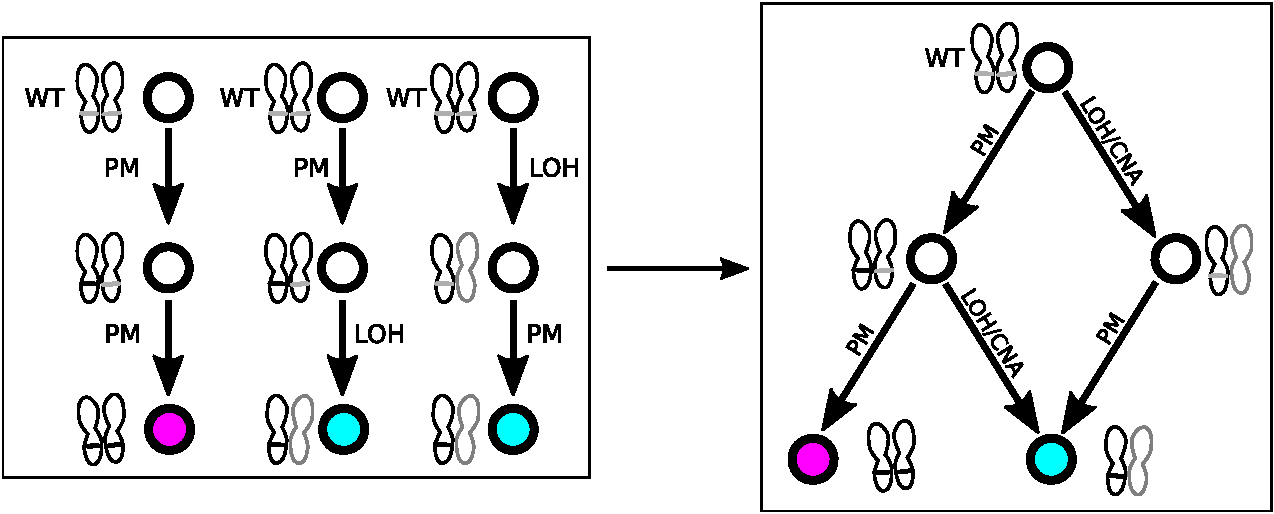
\includegraphics[width=1.0\textwidth]{figures/diagram4b}
    \end{center}
    \begin{columns}
        \begin{column}{0.12\textwidth}
        \begin{center}
            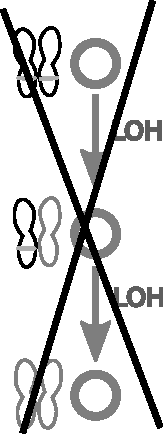
\includegraphics[width=0.75\textwidth]{figures/forbidden}
        \end{center}
        \end{column}
        \begin{column}{0.88\textwidth}
        $\leftarrow$ this order of events is impossible

        (resulting cells are non-viable)
        \end{column}
    \end{columns}
\end{frame}

\begin{frame}
    \frametitle{Network models}
    \framesubtitle{Worked example: tumour suppressor loss-of-function}
    % Now we give each mechanism/event a rate
    \begin{columns}
        \begin{column}{0.5\textwidth}
        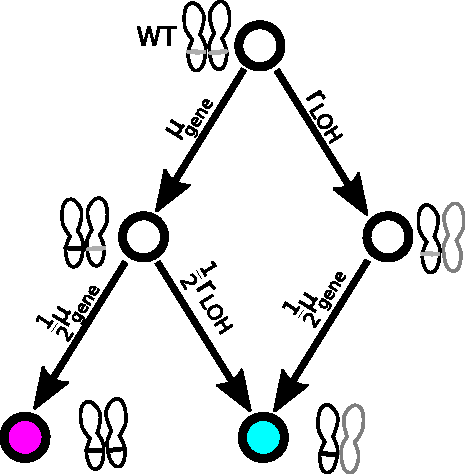
\includegraphics[width=\textwidth]{figures/diagram4c}
        \end{column}
        \begin{column}{0.5\textwidth}
            Assign rates to events:
        \begin{itemize}
            \item Get $\mu_{gene}$ from $n_{gene} \times u \times b$
            \item To get $n_{gene}$, count possible nonsense codons in a
            known sequence
            \item Fix $r_{LOH}$ by looking at relative frequency of LOH
        \end{itemize}
        \end{column}
    \end{columns}
\end{frame}


\begin{frame}
    \frametitle{Colorectal adenocarcinoma model}
    % two TSes lost one oncogene gained
    % product of three graphs: each gene has independent dynamics
    % successfully bound epistasis!
    \begin{center}
        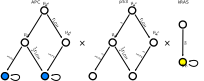
\includegraphics[width=1.0\textwidth]{figures/diagram5}
    \end{center}

    \begin{center}
    \begin{itemize}
        \item \emph{APC-p53-kRAS} combo accounts for about $15\%$ of incidence
        \item 5-year survival about $60\%$ (any stage)
    \end{itemize}
    \end{center}

\footnotetext[1]{Fearon et~al. TODO}
\footnotetext[1]{M. S. Lawrence et~al., Nature 2014; 505: 495–501}
\footnotetext[2]{Office for National Statistics, England 2019}
% Fearon et al on the route
\end{frame}

\begin{frame}
    \frametitle{Colorectal adenocarcinoma model}
    \framesubtitle{Simplified}

    \begin{center}
        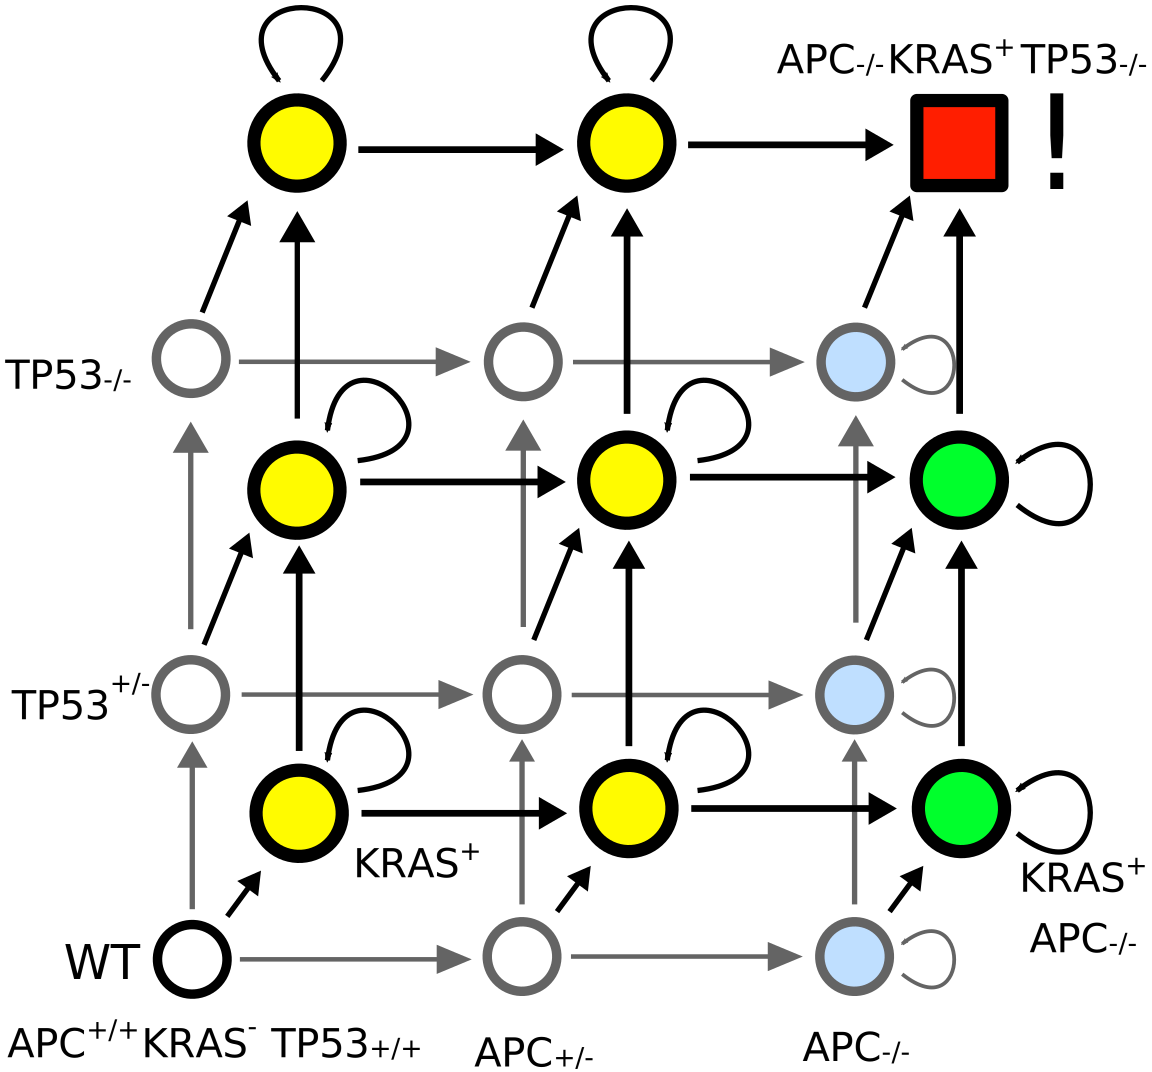
\includegraphics[height=0.8\textheight]{figures/cubegraph4-3}
    \end{center}
\end{frame}
% maybe one slide dedicated to the actual graph (generate programmatically) in
% all its 50-dimensional glory

\begin{frame}
    \frametitle{Colorectal adenocarcinoma model}
    \begin{center}
        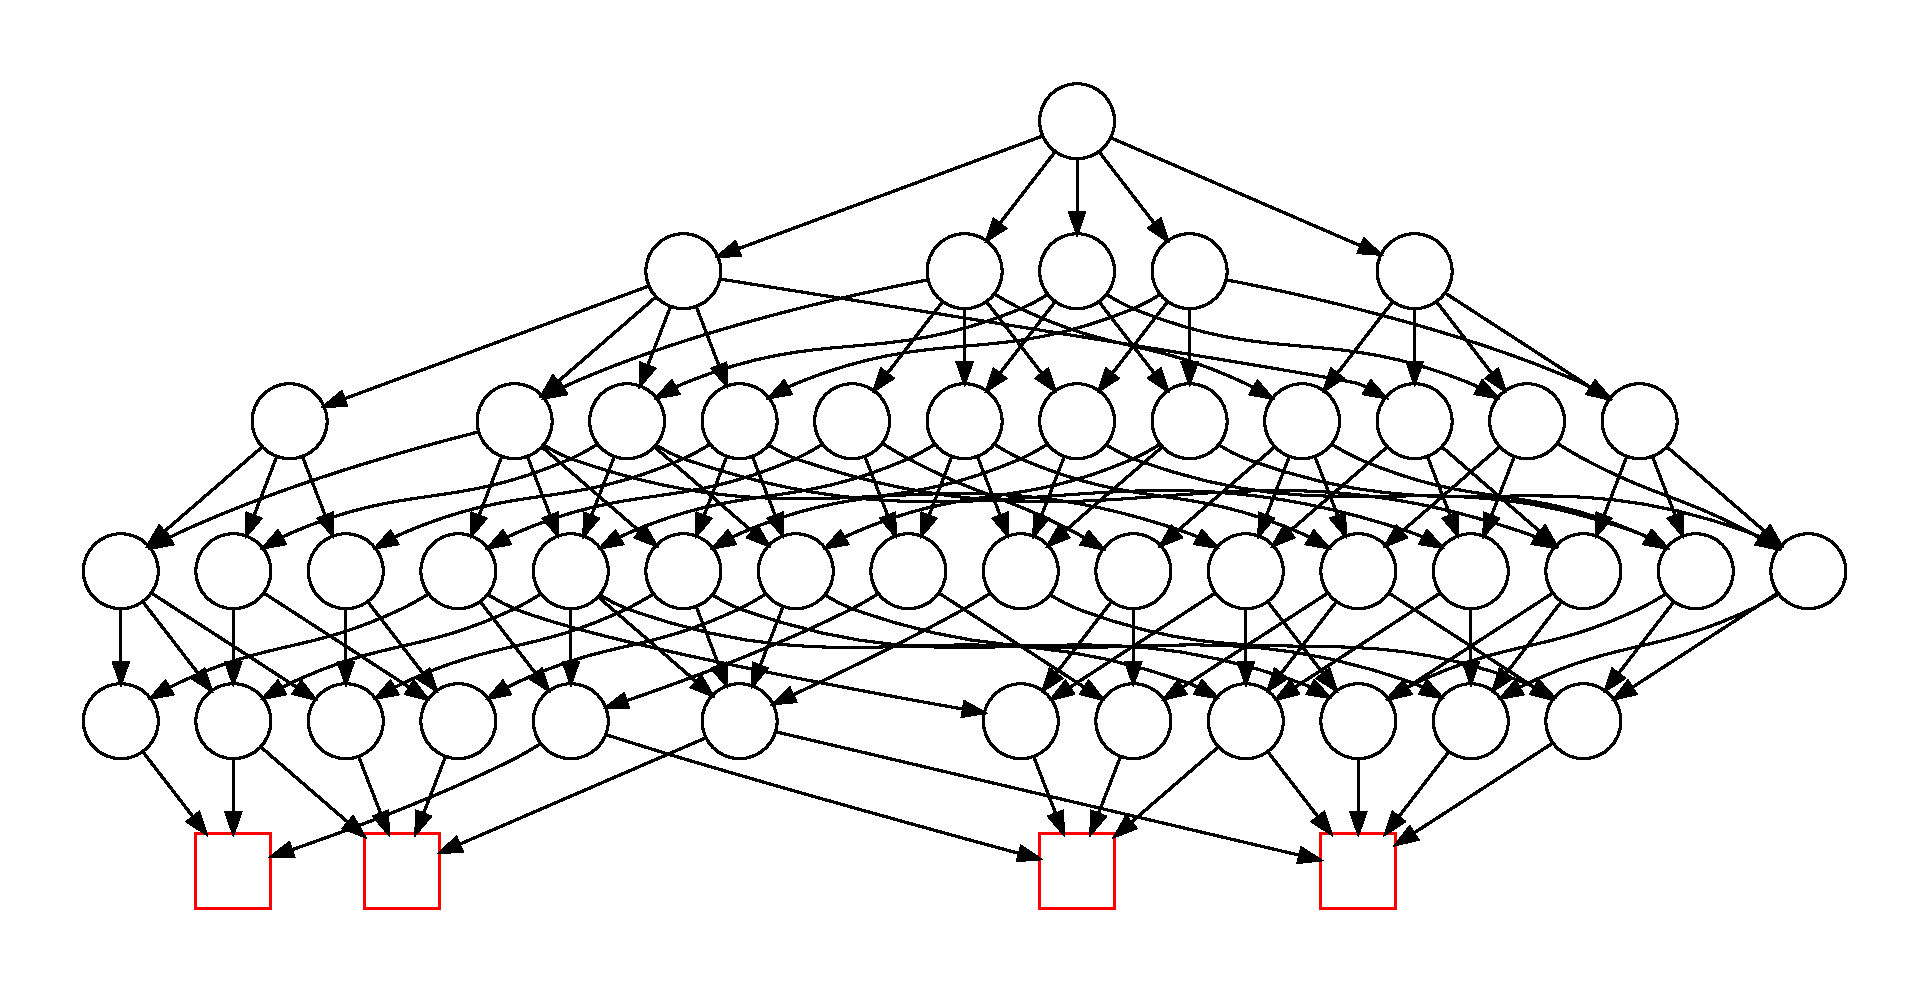
\includegraphics[width=1.0\textwidth]{figures/diagram6}
    \end{center}


    \begin{center}
        \small{each end node is a different copy number profile}

        \;

        \small{e.g. $(-17p, -5q)$, etc}
    \end{center}
\footnotetext[1]{C. Paterson, I. Bozic, H. Clevers, PNAS 2020; 117(34):
20681-20688 (supp. material)}
\end{frame}

\begin{frame}
    \frametitle{Colorectal adenocarcinoma model}

    \begin{center}
        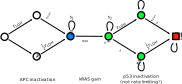
\includegraphics[width=1.0\textwidth]{figures/diagram7}
    \end{center}

    \begin{equation*}
        P(t) \sim t e^{s_2 t}
    \end{equation*}
    \begin{center}
    \begin{itemize}
        \item The $4$ most likely paths account for $50\%$ of the risk
        \item Consistent with classic model\footnotemark[2]
    \end{itemize}
    \end{center}
\footnotetext[1]{C. Paterson, I. Bozic, H. Clevers, PNAS 2020; 117(34): 20681-20688}
\footnotetext[2]{Kinzler and Vogelstein 1990}
\end{frame}
% The solution method is more interesting than the actual solution, but can show
% some very important (most likely!) paths and the corresponding curve

\begin{frame}
    \frametitle{Colorectal adenocarcinoma model}
    \framesubtitle{Successful \emph{ab initio} model}
    \begin{columns}
        \begin{column}{0.5\textwidth}
        % graph from our PNAS paper
        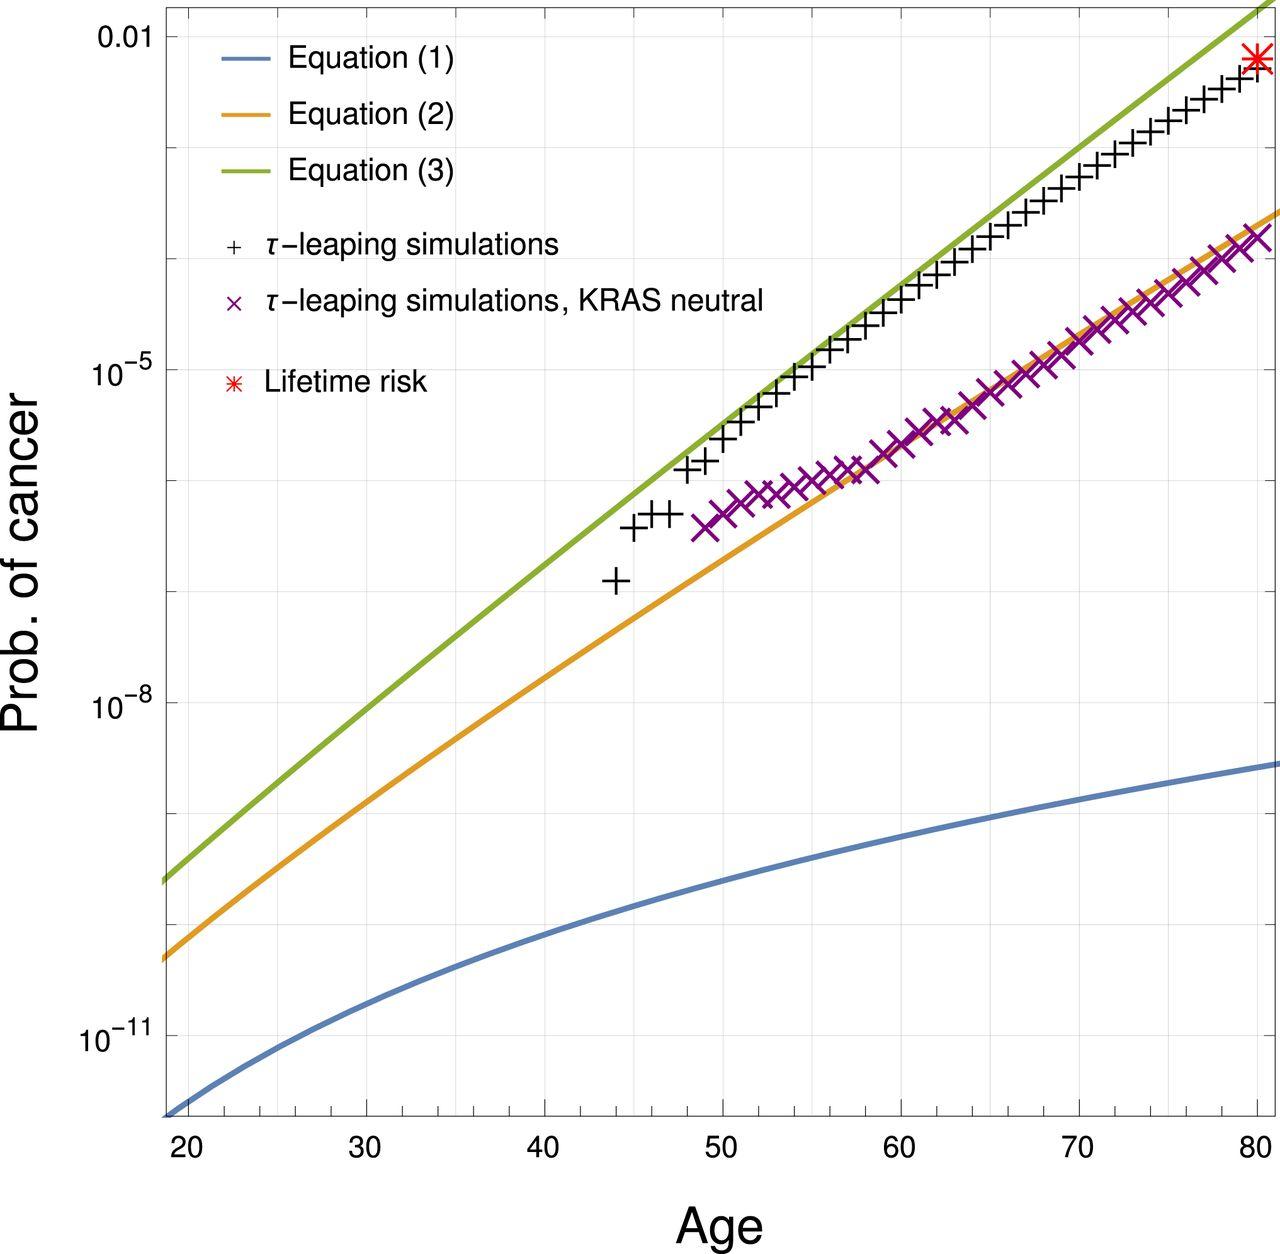
\includegraphics[width=\textwidth]{figures/F2.large.jpg}
        \end{column}
        \begin{column}{0.5\textwidth}
        \begin{itemize}
            \item Gets proportion of incidence right -- \emph{with no fitting!}
            \item Can constrain \emph{APC/KRAS} epistasis ($s_{2} < 0.31$/yr)
            \item Timing of \emph{p53} inactivation: must be \emph{late}${}^2$
            \item \emph{Compatible with} 3-hit models, similar curve: 
                  \emph{p53 not rate limiting}
            \item Conditional path probabilities $P(X_i)$ encode fitnesses
        \end{itemize}
        \end{column}
    \end{columns}
\footnotetext[1]{C. Paterson, I. Bozic, H. Clevers, PNAS 2020; 117(34): 20681-20688}
\footnotetext[2]{(relative to the others)}
\end{frame}

\begin{frame}
    \frametitle{Colorectal adenocarcinoma model}
    \framesubtitle{Science is very hard}
    % Some problems with this model
    % picture of the Sun, glaring
    \begin{enumerate}
        \item model only accounts for $15\%$ of lifetime risk${}^{1,2}$
        \item often malignant on discovery: difficult to constrain
        timing${}^3$ or effect of drivers 
        % 175 - 55 = 120
        \item 5 hits, 50 nodes, 120 edges, 270 paths, strong selection: complicated
        \item approximations inaccurate when probabilities large
    \end{enumerate}


\footnotetext[1]{M. S. Lawrence et~al., Nature 2014; 505: 495–501}
\footnotetext[2]{C. Paterson, I. Bozic, H. Clevers, PNAS 2020; 117(34): 20681-20688}
\footnotetext[3]{(relative to malignant transformation)}
% Fearon et al on the route
\end{frame}
{
\setbeamertemplate{background}
{
    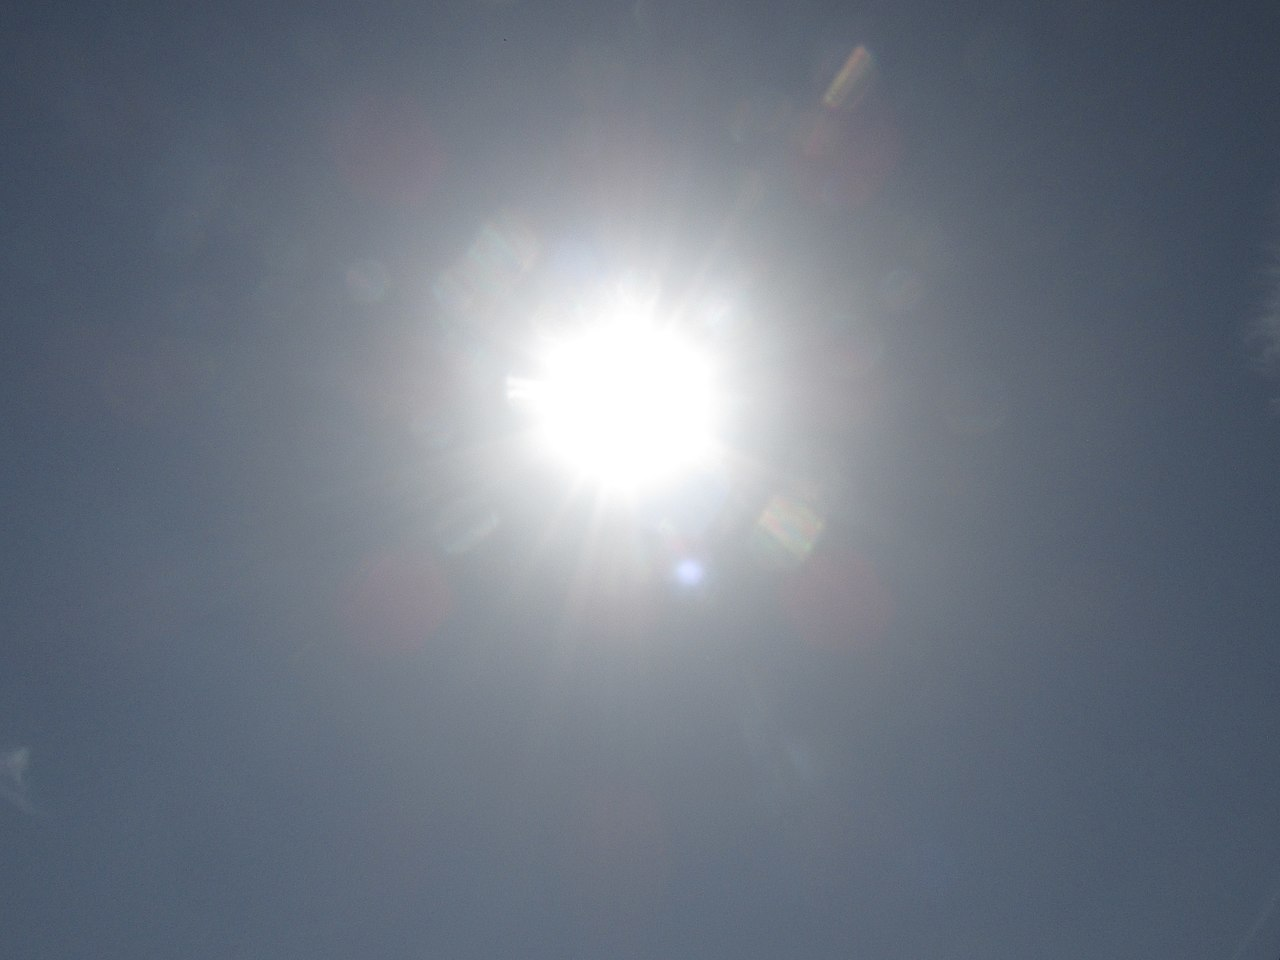
\includegraphics[width=\paperwidth]{figures/1280px-Sun_(Earth_POV).jpg}
}
\begin{frame}
    \frametitle{}
    \begin{center}
        common and malignant = difficult to study
    \end{center}

\footnotetext[1]{https://commons.wikimedia.org/wiki/File:Sun\_(Earth\_POV).jpg}
\end{frame}
}


% Why study schwannoma?

\begin{frame}
    \frametitle{Why study vestibular schwannoma?}
    \framesubtitle{Sometimes rare events make more interesting science possible}
    % Sometimes RARE EVENTS make more interesting science possible
    % Solar eclipse picture

    \begin{enumerate}
        \item genomic subtypes better characterised: \emph{NF2/Merlin}
        altered in $85-100\%$ of cases${}^{1,2}$, \emph{TP53} in
        $\approx 0\%$
        \item usually benign = \textbf{easier to study timing!} (of drivers,
        malignant transformation...)
        \item only 3 hits, weak selection (almost neutral)
        \item probabilities low: approximations v. accurate \textbf{because it's rare}
    \end{enumerate}


% interestingly, TP53 LOF is extremely rare

\footnotetext[1]{ML Carlson et~al., Otology \& Neurotology: 2018;39(9):860 -- 871}
\footnotetext[2]{AL Håvik et~al., Journal of Neurosurgery JNS. 2017;128(3):911 -- 922.}
\newblock 
\newblock 

\end{frame}

{
\DarkMode
\setbeamertemplate{background}
{
    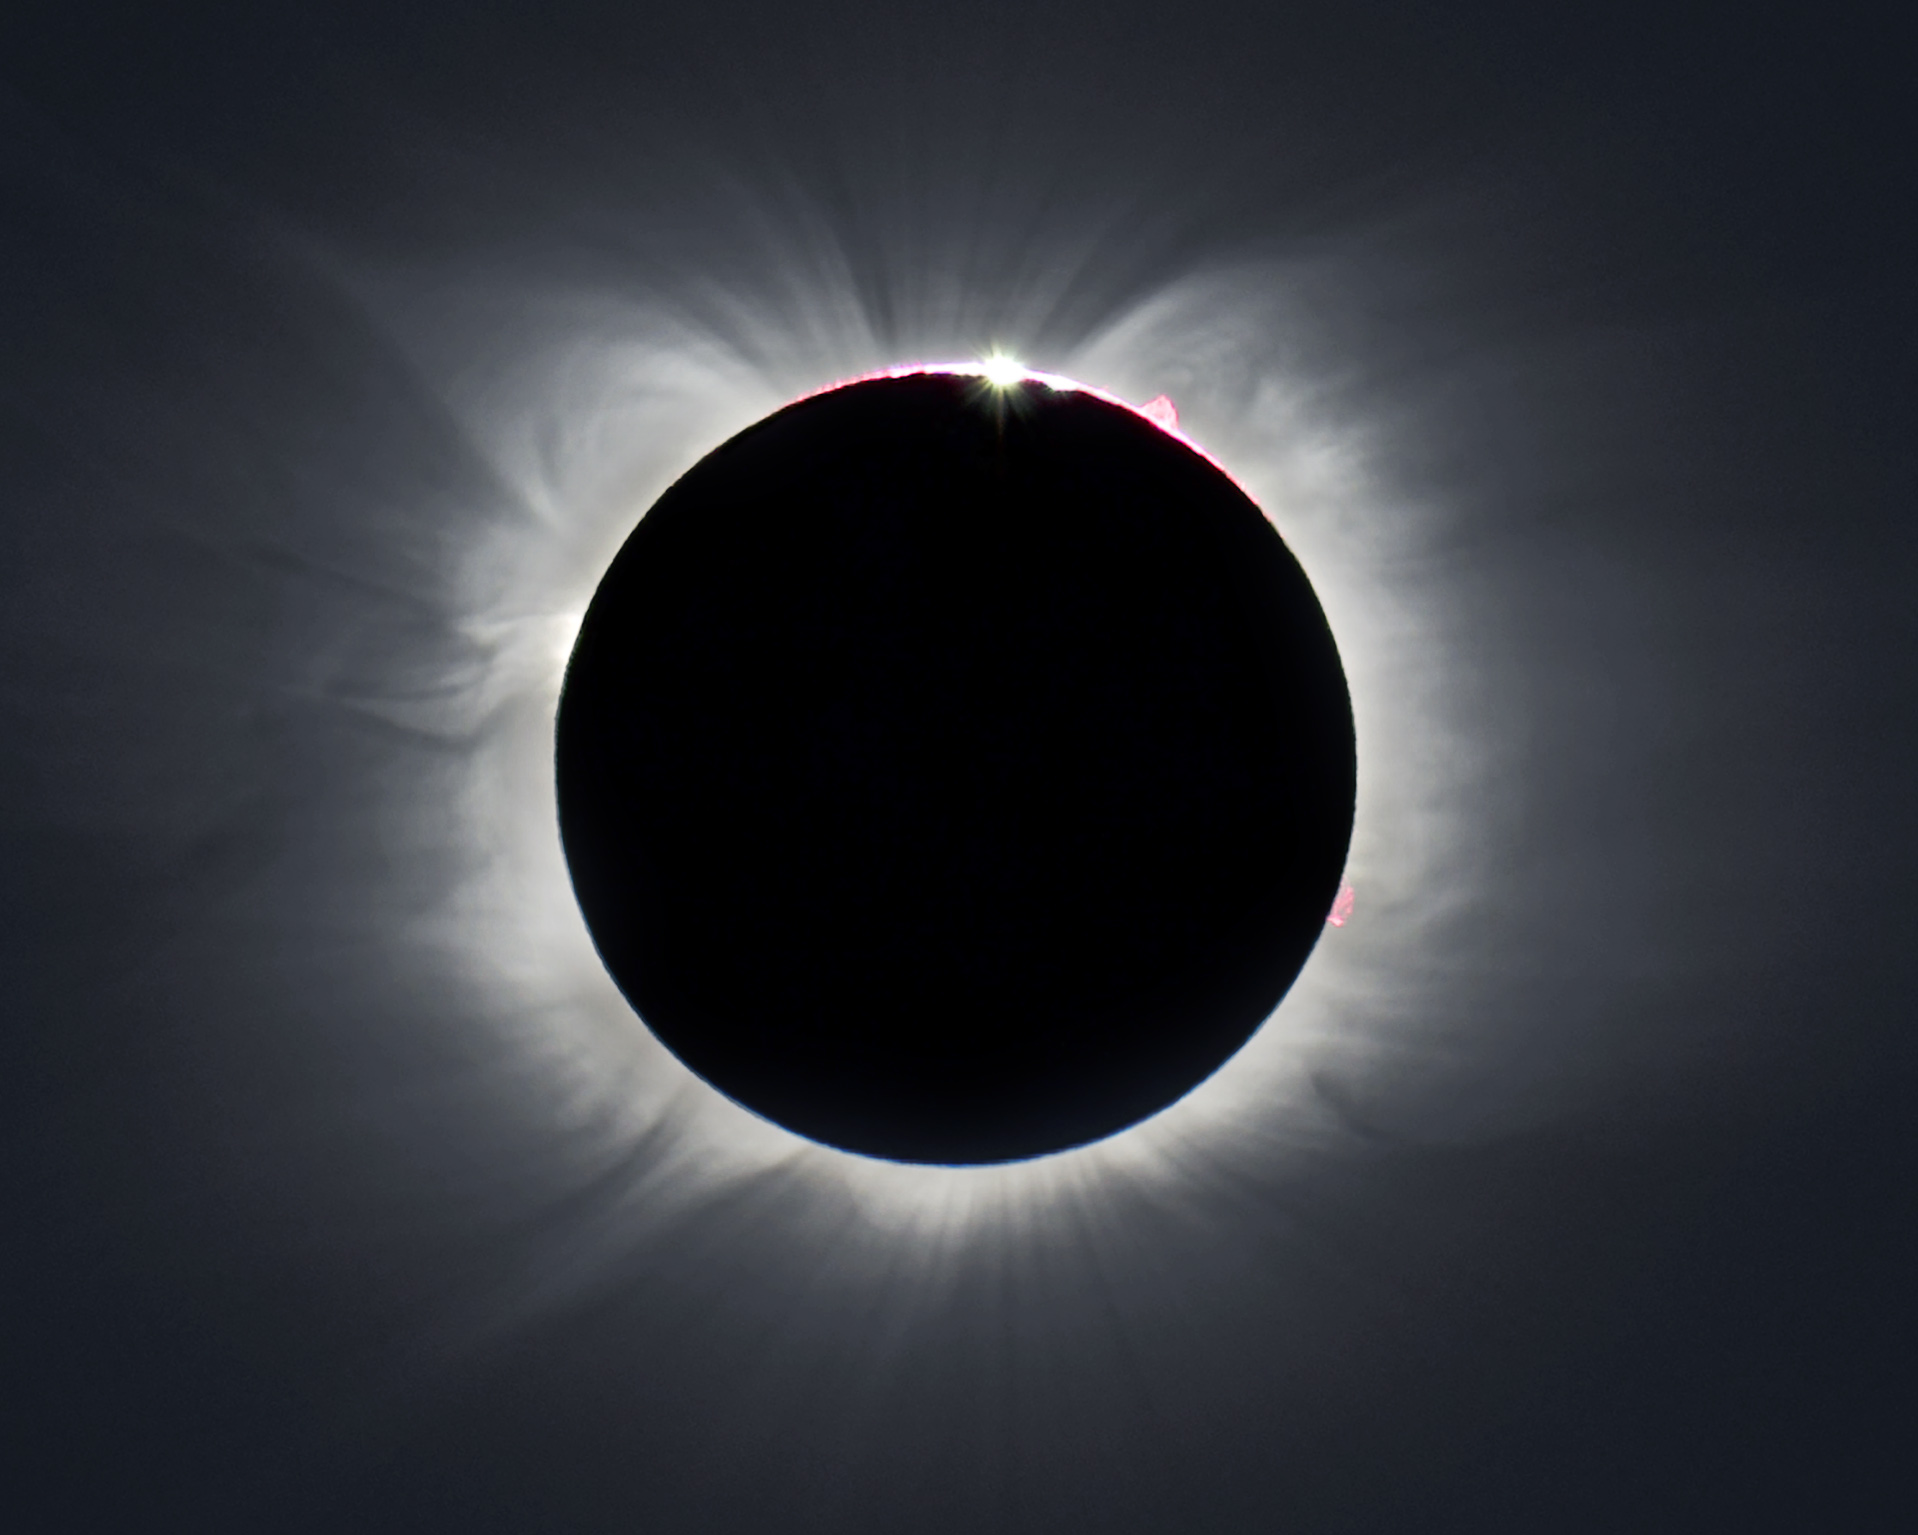
\includegraphics[width=1.0\paperwidth]{figures/SOLARECLIPSE2021FORDISTROHighRes.jpg}
}
\begin{frame}
    \frametitle{}

    \;

    \;

    \;

\begin{center}
    \contour{black}{rare and benign}

    +

    \contour{black}{ high quality data}
\end{center}
\footnotetext[1]{https://apod.nasa.gov/apod/ap211209.html}
\end{frame}
}

\begin{frame}
    \frametitle{Vestibular schwannoma}
    \framesubtitle{3-\emph{event} model}
    % picture of Woods model and a graph
    % O --> O --> O! 2 stage in NF2, 3 hit (rel. to WT/GP)
    % include loops for rigour w/correct alpha and beta
    % very low fitness: s ~ 0.005 /yr

    \begin{columns}
        \begin{column}{0.5\textwidth}
        %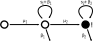
\includegraphics[width=0.99\textwidth]{figures/diagramwoods}
        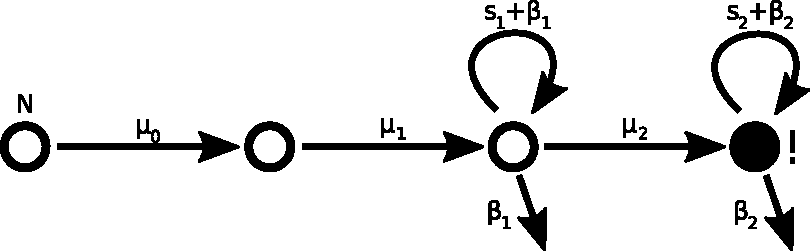
\includegraphics[width=0.99\textwidth]{figures/diagram3}

        \begin{itemize}
            \item Fitness suspiciously low, $s \approx 0.005$/yr
            \footnotemark[1]
            \item Suggests nearly-neutral 3-hit model
            \footnotemark[3]
        \end{itemize}
        \end{column}
        \begin{column}{0.5\textwidth}
        % TODO replace with Evans 2005 (our data!) !!!
        % graph with our model/data
        % Graph with incidence?
        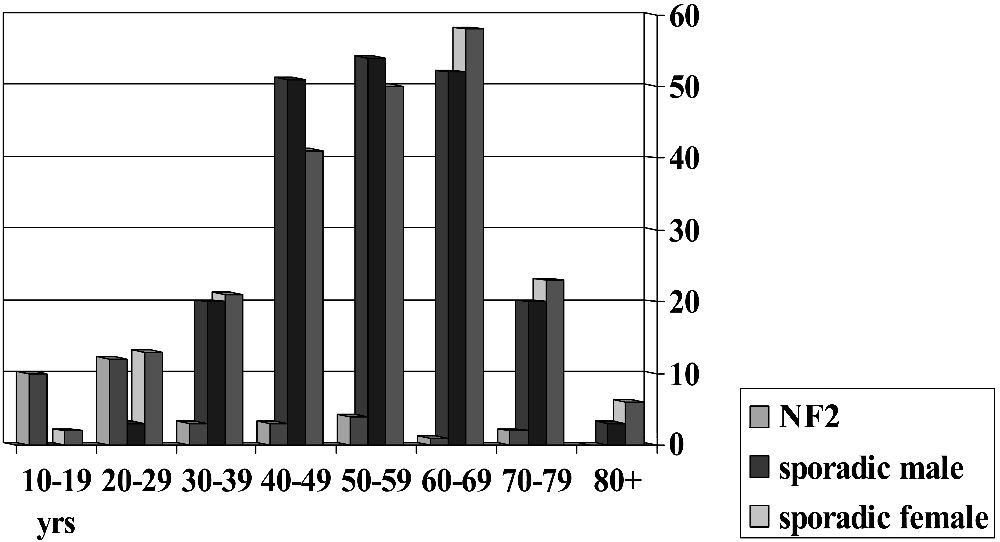
\includegraphics[width=0.99\textwidth]{figures/DGREvans2005}
        \end{column}
    \end{columns}

\footnotetext[1]{R. Woods \emph{et al.} Genetic Epidemiology (2003)24: 265–272}
\footnotetext[2]{DGR. Evans \emph{et al.} Otology \& Neurotology (2005)26:93–97}
\footnotetext[3]{\tiny{C Paterson, I Bozic, MJ Smith, X Hoad, DGR Evans,
 https://doi.org/10.1101/2021.10.03.457528}}
% Evans 2005
\end{frame}

% DGR Evans 2005
% 3 hit model

\begin{frame}
    \frametitle{Vestibular schwannoma incidence}
    \framesubtitle{Our model for sporadic VS}
    % Include LINKAGE of SMARCB1 and NF2

    \begin{columns}
        \begin{column}{0.5\textwidth}
        \begin{itemize}
            \item Include \emph{NF2}, \emph{SMARCB1} and (simplified) linkage
            \item Add hypothetical oncogene \emph{GFX}
            % really n_GFX is all the sensitive sites on many possible third
            % hits
        \end{itemize}

        \;
        % Point out TS loss motif of NF2
        % Graph of actual incidence on left

        Risk of each subtype looks like

    \begin{equation*}
        P(\mathrlap{\textcolor{cyan}{\blacksquare}}\Box) \propto \frac{t^3}{3!}
    \end{equation*}
    \begin{equation*}
        \vphantom{P(\mathrlap{\textcolor{cyan}{\blacksquare}}\Box) \approx N_{WT} \mu_{GFX}
        r_{LOH} \frac{1}{2} \mu_{NF2} \frac{t^3}{3!}  \times 6}
    \end{equation*}
        \end{column}
        \begin{column}{0.5\textwidth}
        \begin{center}
            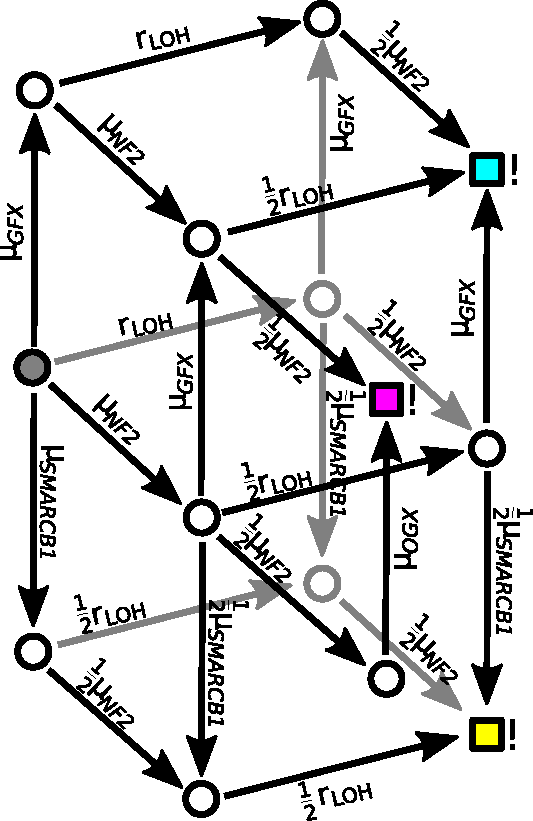
\includegraphics[height=0.8\textheight]{figures/vsmodel-nochromosomes.pdf}
        \end{center}
        \end{column}
    \end{columns}
    
    % Should explain around 80% of incidence well, huge improvement on CRC
    % model
\footnotetext[1]{\tiny{C Paterson, I Bozic, MJ Smith, X Hoad, DGR Evans,
 https://doi.org/10.1101/2021.10.03.457528}}
\end{frame}

\begin{frame}
    \frametitle{Vestibular schwannoma incidence}
    \framesubtitle{Our model for sporadic VS}
    % 3 hit model following Woods
    % Include LINKAGE of SMARCB1 and NF2

    \begin{columns}
        \begin{column}{0.5\textwidth}
        \begin{itemize}
            \item Include \emph{NF2}, \emph{SMARCB1} and (simplified) linkage
            \item Add hypothetical oncogene \emph{GFX}
        \end{itemize}

        \;
        % Diagram of our model
        % Point out TS loss structure of NF2
        % Graph of actual incidence on left

        Risk of each subtype looks like

    \begin{equation*}
        P(\mathrlap{\textcolor{cyan}{\blacksquare}}\Box) \propto \frac{t^3}{3!}
    \end{equation*}
    \begin{equation*}
        P(\mathrlap{\textcolor{cyan}{\blacksquare}}\Box) \approx N_{WT} \mu_{GFX}
        r_{LOH} \frac{1}{2} \mu_{NF2} \frac{t^3}{3!}  \times 6
    \end{equation*}
        \end{column}
        \begin{column}{0.5\textwidth}
        \begin{center}
            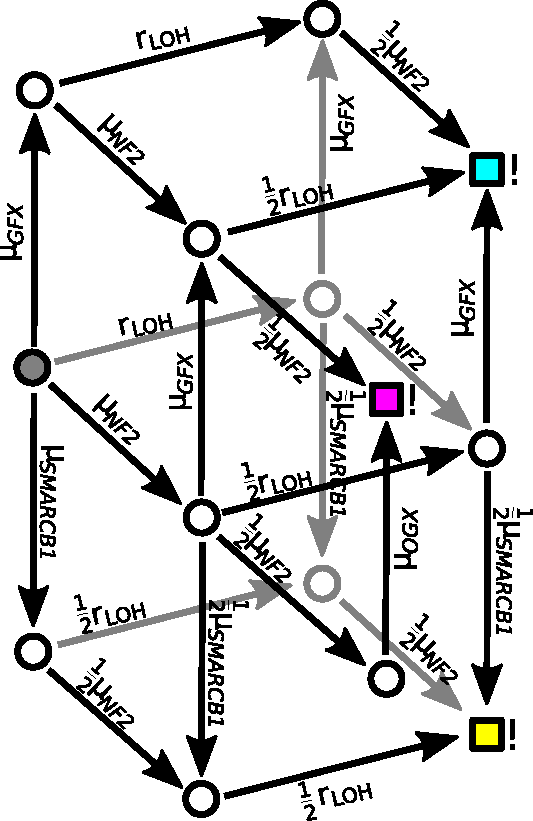
\includegraphics[height=0.8\textheight]{figures/vsmodel-nochromosomes.pdf}
        \end{center}
        \end{column}
    \end{columns}
    
    % Should explain around 80% of incidence well, huge improvement on CRC
    % model
\footnotetext[1]{\tiny{C Paterson, I Bozic, MJ Smith, X Hoad, DGR Evans, https://doi.org/10.1101/2021.10.03.457528}}
\end{frame}


\begin{frame}
    \frametitle{Vestibular schwannoma incidence}
    \framesubtitle{Our model for sporadic VS}
    \begin{columns}
        \begin{column}{0.5\textwidth}
            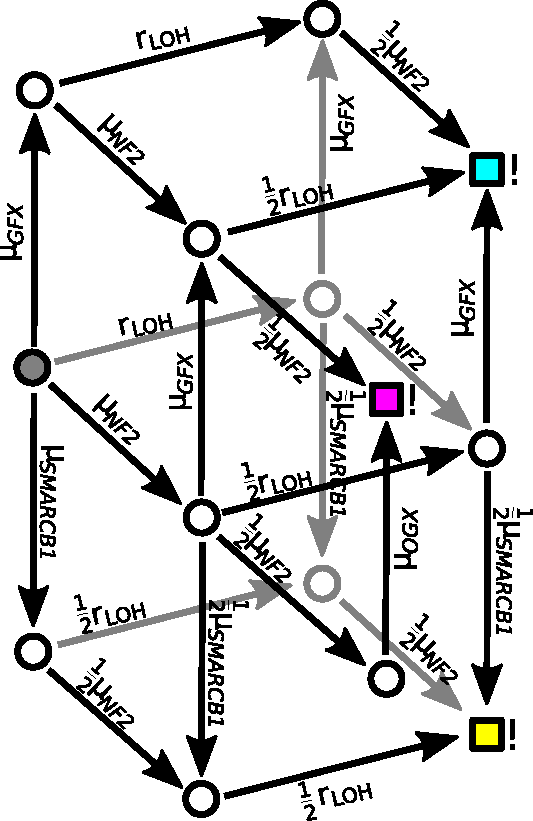
\includegraphics[height=0.8\textheight]{figures/vsmodel-nochromosomes.pdf}
        \end{column}
        \begin{column}{0.5\textwidth}
        \begin{itemize}
            \item $\mathrlap{\textcolor{cyan}{\blacksquare}}\Box +
            \mathrlap{\textcolor{yellow}{\blacksquare}}\Box$ = have LOH on 22q
            \item frequency of LOH = $f_{LOH} = (
            \mathrlap{\textcolor{cyan}{\blacksquare}}\Box
            + 
            \mathrlap{\textcolor{yellow}{\blacksquare}}\Box
            )/(
            \mathrlap{\textcolor{cyan}{\blacksquare}}\Box
            + 
            \mathrlap{\textcolor{yellow}{\blacksquare}}\Box
            + 
            \mathrlap{\textcolor{magenta}{\blacksquare}}\Box
            )$
            \item $\mathrlap{\textcolor{yellow}{\blacksquare}}\Box$ =
            \emph{SMARCB1}${}^{-/-}$
            \item frequency of \emph{SMARCB1}${}^{-/-}$ = $f_{SMARCB1}$

            \;

            $= \mathrlap{\textcolor{yellow}{\blacksquare}}\Box
            /(
            \mathrlap{\textcolor{cyan}{\blacksquare}}\Box
            + 
            \mathrlap{\textcolor{yellow}{\blacksquare}}\Box
            + 
            \mathrlap{\textcolor{magenta}{\blacksquare}}\Box
            )$

        \end{itemize}

        Can use these to fix parameters!
        \end{column}
    \end{columns}

    % interesting: could try fixing fSMARCB1 from looking at tumours WITH
    % LOH(22q) but WITHOUT additional insults to NF2, and assuming the VAF
    % detected is uncharacterised pathology? Ask Miriam.
\end{frame}

\begin{frame}
    \frametitle{Vestibular schwannoma incidence}
    \framesubtitle{Our model for sporadic VS}
    \begin{columns}
        \begin{column}{0.5\textwidth}
        \begin{itemize}
            \item \emph{Don't} use \emph{ab initio} point estimates for $u$, $r_{LOH}$, $n_{GFX}$ this time...
            \item Instead use $P(t) = \mathrlap{\textcolor{cyan}{\blacksquare}}\Box
            + 
            \mathrlap{\textcolor{yellow}{\blacksquare}}\Box
            + 
            \mathrlap{\textcolor{magenta}{\blacksquare}}\Box$, $f_{LOH} =
            \frac{
            \mathrlap{\textcolor{cyan}{\blacksquare}}\Box
            + 
            \mathrlap{\textcolor{yellow}{\blacksquare}}\Box
            }{
            \mathrlap{\textcolor{cyan}{\blacksquare}}\Box
            + 
            \mathrlap{\textcolor{yellow}{\blacksquare}}\Box
            + 
            \mathrlap{\textcolor{magenta}{\blacksquare}}\Box
            }$, and
            $f_{SMARCB1}= 
            \frac{
            \mathrlap{\textcolor{yellow}{\blacksquare}}\Box
            }{
            \mathrlap{\textcolor{cyan}{\blacksquare}}\Box
            + 
            \mathrlap{\textcolor{yellow}{\blacksquare}}\Box
            + 
            \mathrlap{\textcolor{magenta}{\blacksquare}}\Box
            }$ to fix the parameters!
        \end{itemize}
        \end{column}
        \begin{column}{0.5\textwidth}
            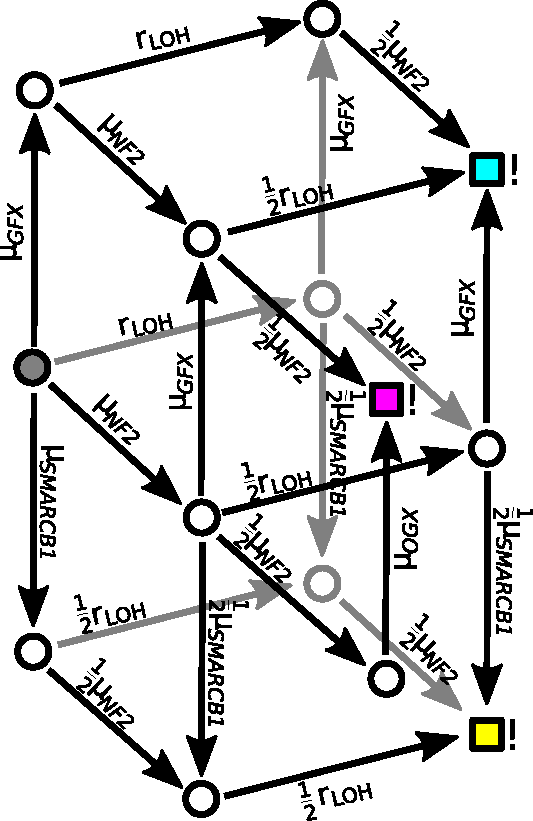
\includegraphics[height=0.8\textheight]{figures/vsmodel-nochromosomes.pdf}
        \end{column}
    \end{columns}
\end{frame}


\begin{frame}
    \frametitle{Vestibular schwannoma incidence}
    \framesubtitle{Our model for sporadic VS}
    \begin{columns}
        \begin{column}{0.5\textwidth}
            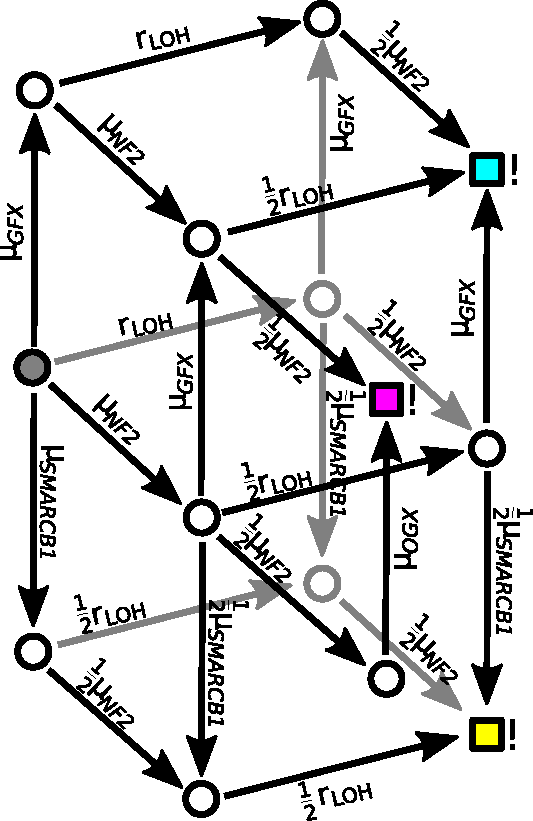
\includegraphics[height=0.8\textheight]{figures/vsmodel-nochromosomes.pdf}
        \end{column}
        \begin{column}{0.5\textwidth}
            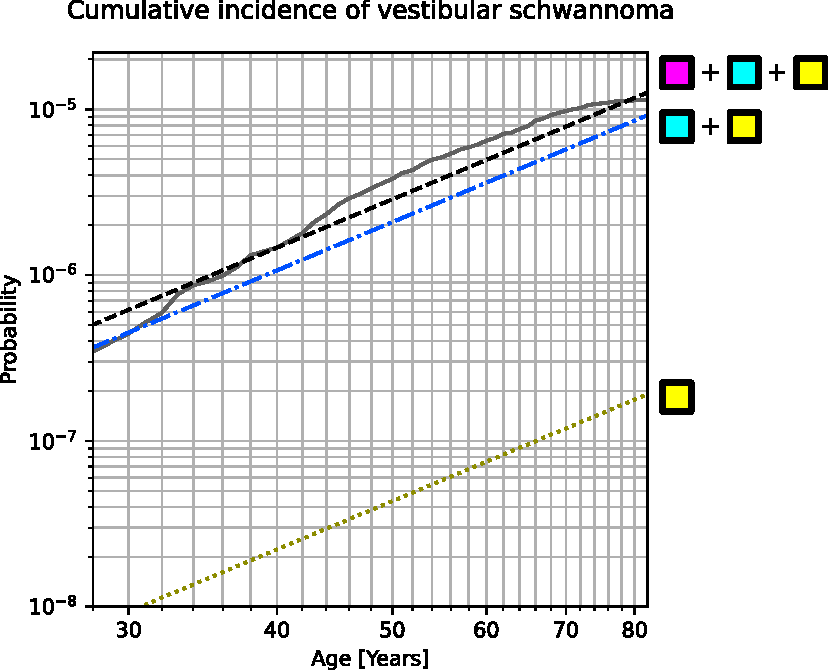
\includegraphics[width=1.0\textwidth]{figures/figure-5-3Hit-feb22}
        \end{column}
    \end{columns}
\footnotetext[1]{\tiny{C Paterson, I Bozic, MJ Smith, X Hoad, DGR Evans, https://doi.org/10.1101/2021.10.03.457528}}
\end{frame}

\begin{frame}
    \frametitle{Vestibular schwannoma incidence}
    \framesubtitle{New parameter estimates}
    % Figures from paper? i.e. bootstrapped distributions

    \begin{center}
    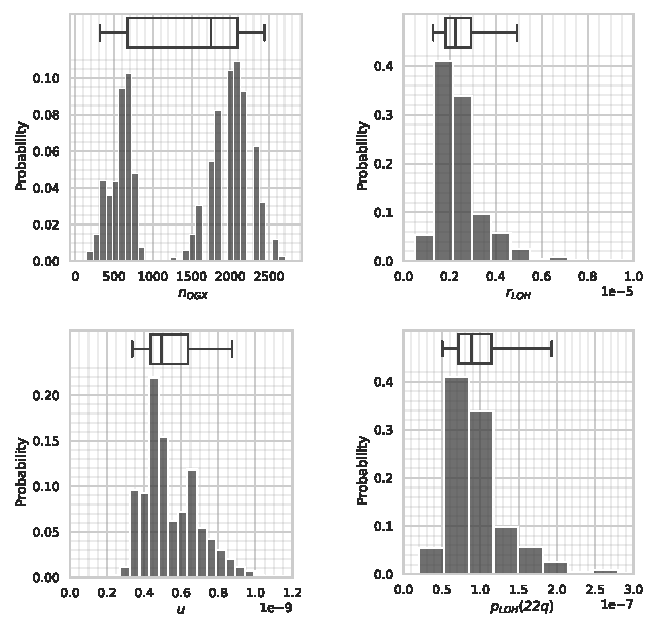
\includegraphics[height=0.85\textheight]{figures/Fig3-combined-bw-feb22}

    \;

        \tiny{bootstrapped distributions}
    \end{center}
\end{frame}


\begin{frame}
    \frametitle{Malignant transformation in vestibular schwannoma}
    \framesubtitle{Very rare, very bad}
            \begin{itemize}
                \item Risk $\approx 0.1\%$ of VS cases
                \item 5-year survival $\approx 12-20\%$
            \end{itemize}
    \begin{columns}
        \begin{column}{0.5\textwidth}
        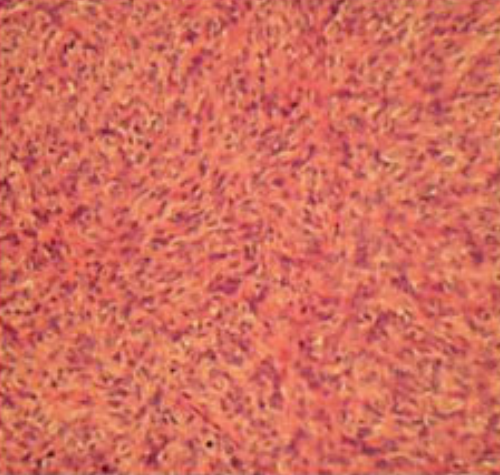
\includegraphics[width=\textwidth]{figures/AKDemetriades_Fig5C.png}
        \end{column}
        \begin{column}{0.5\textwidth}
        % histological slide of an MPNST
        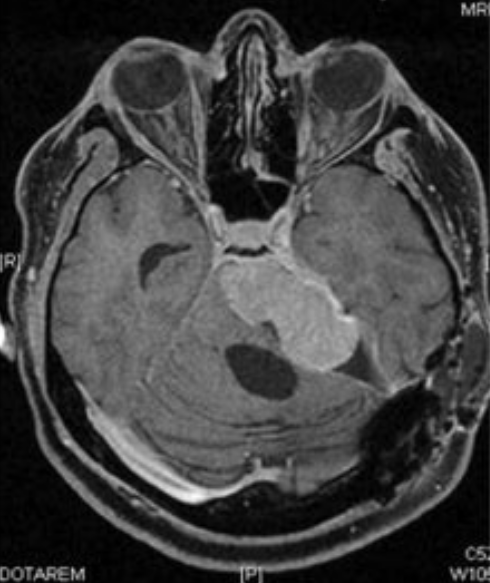
\includegraphics[width=\textwidth]{figures/AKDemetriades_Fig4C.png}
        \end{column}
    \end{columns}
\footnotetext{AK Demetriades et~al. Skull Base (2010)20:381–387.}%http://dx.doi.org/10.1055/s-0030-1253576}
\end{frame}

\begin{frame}
    \frametitle{Malignant schwannoma: two models}
    \framesubtitle{Timing and identity of drivers}
    % Very rare
    % Malignant transformation not well understood in general

    \begin{columns}
        \begin{column}{0.5\textwidth}
        % DIAGRAM
        Oncogene activation: %$\implies$ high risk
        \end{column}
        \begin{column}{0.5\textwidth}
        % OG graph, need to remake TODO
        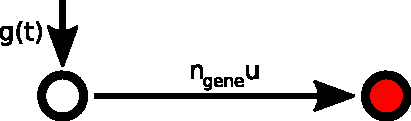
\includegraphics[width=\textwidth]{figures/malignancy-oncogene.pdf}
        \end{column}
    \end{columns}

    \;

    \begin{columns}
        \begin{column}{0.5\textwidth}
        % DIAGRAM
        \emph{TSX} inactivation: %$\implies$ low risk
        \end{column}
        \begin{column}{0.5\textwidth}
        % TS graph, from main paper
        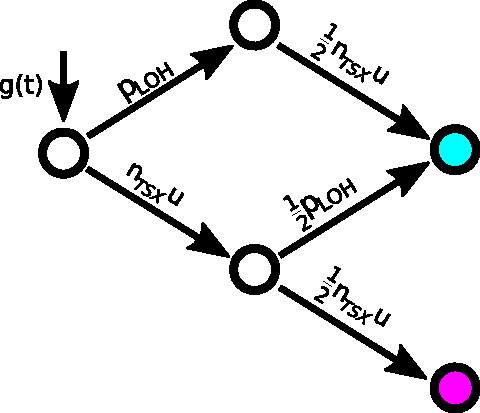
\includegraphics[width=\textwidth]{figures/malignancy.pdf}
        \end{column}
    \end{columns}
    %(Much more likely!)

    %\;

    \begin{center}
        Malignant VS is \emph{extremely} rare!
    \end{center}

\footnotetext[1]{\tiny{C Paterson, I Bozic, MJ Smith, X Hoad, DGR Evans, https://doi.org/10.1101/2021.10.03.457528}}
\end{frame}

\begin{frame}
    \frametitle{Malignant schwannoma: first model}
    \framesubtitle{Oncogene activation}
    \begin{columns}
        \begin{column}{0.5\textwidth}
        % DIAGRAM
        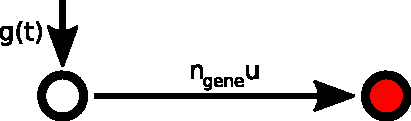
\includegraphics[width=\textwidth]{figures/malignancy-oncogene.pdf}
        \end{column}
        \begin{column}{0.5\textwidth}
        % OG graph, TODO NEED TO REMAKE! Ck values of nx!
        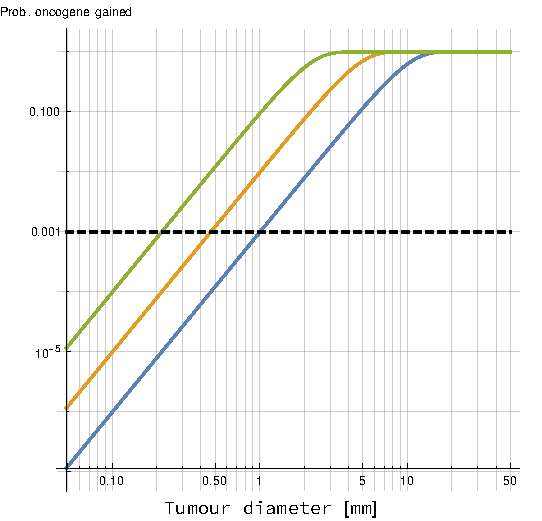
\includegraphics[width=\textwidth]{figures/DiameterOncogene-feb21}
        \end{column}
    \end{columns}

\begin{itemize}
    \item Oncogene activation $\implies$ high risk
    \item But it's a rare outcome
    \item So it's probably not caused by oncogene activation
\end{itemize}

\end{frame}

\begin{frame}
    \frametitle{Malignant schwannoma: second model}
    \framesubtitle{Tumour suppressor \emph{TSX} inactivation}
    \begin{columns}
        \begin{column}{0.45\textwidth}
        % DIAGRAM
        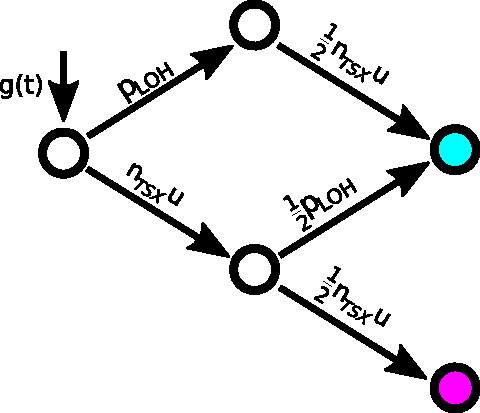
\includegraphics[width=\textwidth]{figures/malignancy.pdf}
        \end{column}
        \begin{column}{0.55\textwidth}
        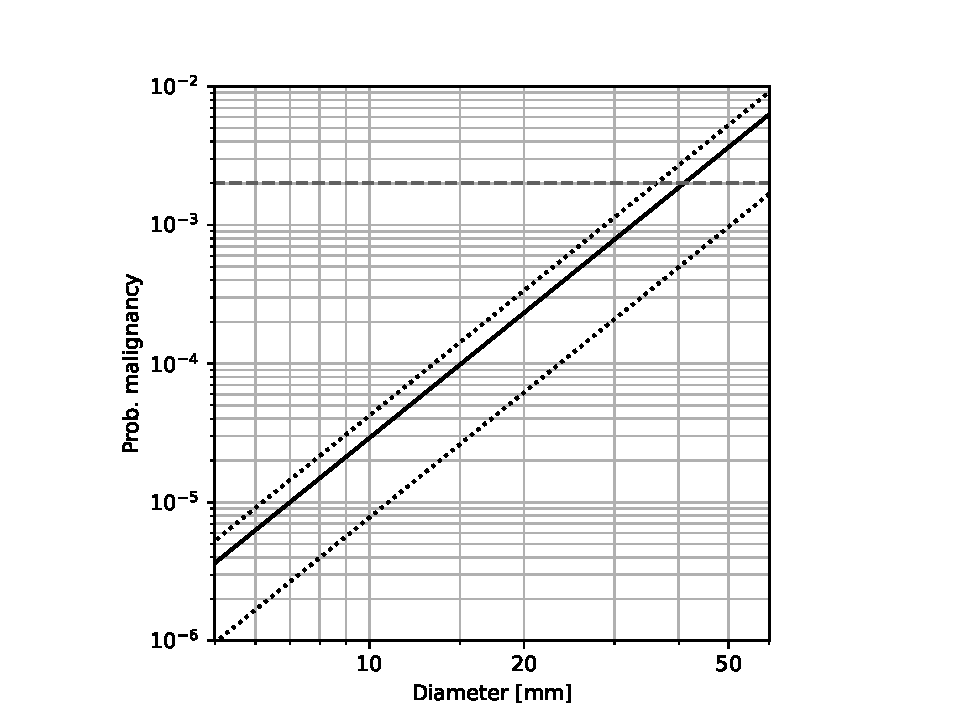
\includegraphics[width=\textwidth]{figures/DiameterTS-oct21}
        \end{column}
    \end{columns}

\begin{itemize}
    \item \emph{TSX} inactivation $\implies$ low risk
    \item Can also estimate $n_{TSX}$ that's consistent with incidence
\end{itemize}
\end{frame}

\begin{frame}
    \frametitle{Who is \emph{TSX}?}
    \framesubtitle{Parameter estimates for $n_{TSX}$}
    % bootstrapped histogram

    \begin{center}
        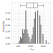
\includegraphics[width=0.5\textwidth]{figures/TSXhistogram}
    \end{center}

    \begin{center}
        \small{Probably multiple (10?) distinct tumour suppressors} 

        \;

        \huge{i.e. not (just) \emph{TP53}: $n_{TP53} = 73$}

        \;

        \small{Disclaimer: assumes neutrality \& haplosufficiency}
    \end{center}

\footnotetext[1]{\tiny{C Paterson, I Bozic, MJ Smith, X Hoad, DGR Evans, https://doi.org/10.1101/2021.10.03.457528}}
\end{frame}

\begin{frame}
    \frametitle{Malignant schwannoma}
    \framesubtitle{Radiation}
    % TODO is this tumour initation or promotion?

    \begin{center}
        \tiny{Why do we care about \emph{TSX} anyway?}
    \end{center}

    \begin{columns}
        \begin{column}{0.5\textwidth}
        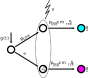
\includegraphics[width=\textwidth]{figures/radiation-model}
        \end{column}
        \begin{column}{0.5\textwidth}
        3 dose-dependent effects:
        \begin{itemize}
            \item DSB induction $p_{DSB}(D)$
            \item DSB misrepair $\varepsilon(D)$
            \item cell survival $S(D)$
        \end{itemize}
        \end{column}
    \end{columns}
\end{frame}

% DSB induction: 
\begin{frame}
    \frametitle{DSB induction model}
    \begin{center}
        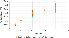
\includegraphics[width=0.75\textwidth]{figures/MObeidat2018}
    \end{center}
\end{frame}

\begin{frame}
    \frametitle{DSB misrepair}

    \begin{itemize}
        \item Should be dose dependent $\varepsilon(D)$...
        \item Maybe also dose-\emph{rate} dependent $\varepsilon(D,\dot{D})$
    \end{itemize}
    \begin{equation*}
        \varepsilon \approx % what did we use
    \end{equation*}
\end{frame}

\begin{frame}
    \frametitle{Cell survival}
    \framesubtitle{}
    \begin{columns}
        \begin{column}{0.5\textwidth}

        \end{column}
    \end{columns}
\end{frame}

\begin{frame}
    \frametitle{Why do we care about \emph{TSX} anyway?}
    Need to know how many indel sites $m_{TSX}$ result in loss of function:

    \begin{equation}
        m_{TSX} \approx 0.42 n_{TSX}
    \end{equation}
\end{frame}

\begin{frame}
    \frametitle{Malignant schwannoma}
    \framesubtitle{Radiation}
    % TODO is this tumour initation or promotion?

    \begin{center}
        \tiny{Why do we care about \emph{TSX} anyway?}
    \end{center}

    \begin{columns}
        \begin{column}{0.5\textwidth}
        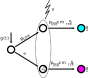
\includegraphics[width=\textwidth]{figures/radiation-model}
        \end{column}
        \begin{column}{0.5\textwidth}
        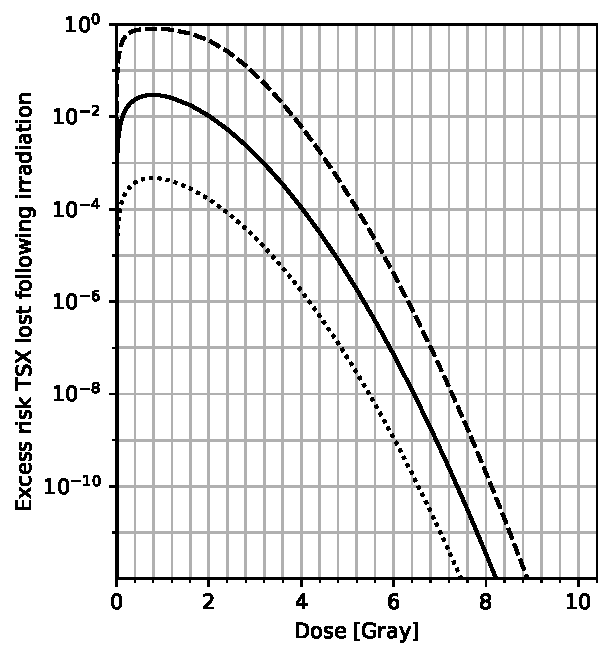
\includegraphics[width=\textwidth]{figures/SecondHitVariousTS-oct21}
        \end{column}
    \end{columns}
\end{frame}


\begin{frame}
    \frametitle{Malignant schwannoma}
    \framesubtitle{Radiation}
    Uncontroversial conclusions, but...

    \begin{itemize}
        \item Model is missing mechanisms (what is $\varepsilon$? multiple genes?)
        \item Multifocality and familial NF2?
        \item Margin clearance \& recurrence?
    \end{itemize}
        \begin{center}
            \emph{What experiments could constrain these?}
        \end{center}
\end{frame}

% TODO skip if preprint not ready
% TODO preprint is definitely not going to be ready
%\begin{frame}
%    \frametitle{DiGeorge syndrome}
%    \framesubtitle{Ongoing work}
%    % copy and paste figures from paper
%    \begin{columns}
%        \begin{column}{0.5\textwidth}
%        % TS loss diagram here
%        \end{column}
%        \begin{column}{0.5\textwidth}
%        % TS loss diagram with forbidden orders
%        % 2 hit diagram
%        \end{column}
%    \end{columns}
%
%    \begin{center}
%        Can (maybe) predict relative risk of schwannoma in rare syndrome
%    \end{center}
%\end{frame}

\begin{frame}
    \frametitle{Main outputs}
    % include a cute diagram
    \begin{enumerate}
        \item Better estimates of event rates in Schwann cells
        \item Can constrain timing of ``\emph{TSX}'' (resp. for malignancy)
        \item Can constrain size of \emph{GFX} and \emph{TSX}
        \item Radiotherapy probably OK (w. caveats + huge error bars)
    \end{enumerate}
\end{frame}

\begin{frame}
    \frametitle{Main outputs}
    but...
    \begin{enumerate}
        \item Uncertainties still large
        \item Identity of \emph{TSX} unknown
        \item Constraints weak: \emph{GFX} and \emph{TSX} probably multiple genes
        \item Don't know about NF2
    \end{enumerate}
\end{frame}

\begin{frame}
    \frametitle{To do list}

    Next gen sequencing...
    \begin{itemize}
        \item Sporadic VS to constrain $f_{SMARCB1}$: $n > 300$
        \item CNA/NGS in MPNST (\textbf{rare!}): $n > 30$
        %\item Study to look at RR in 22q11.2DS: $n > 10000$
        % Not going to be ready
    \end{itemize}

    but also...
    \begin{itemize}
        \item Better models!!! CNA/VAF models, machine learning, optimal clustering, $\mu_{C>T}$ etc.
        \item SEER data too?
        \item Multiple genes \emph{GFX} and \emph{TSX}? 
        \item Haploinsufficiency, selection?
    \end{itemize}
    % more complicated graph

    \begin{center}
        Lots to do!

        \;

        \huge{I need collaborators, send me data}
    \end{center}
\end{frame}

%\begin{frame}
%    \frametitle{The big picture}
%    \framesubtitle{Why study malignant transformation in VS at all}
%    \begin{center}
%        Hi-res look at malignant transformation \emph{in slow motion}, usually
%        impossible!
%    \end{center}
%
%    \begin{center}
%        What genes are responsible? Fundamentally interesting!
%    \end{center}
%    % solar eclipses are rare but resulted in
%    % discovery of helium
%    % discovery of general relativity
%
%% 1868 and 1919
%\end{frame}

%{
% Set colour theme to an ominous white-on-black
\DarkMode
\begin{frame}
    \frametitle{The big picture}
    \framesubtitle{Biology is sometimes compared to physics}

    \begin{center}
        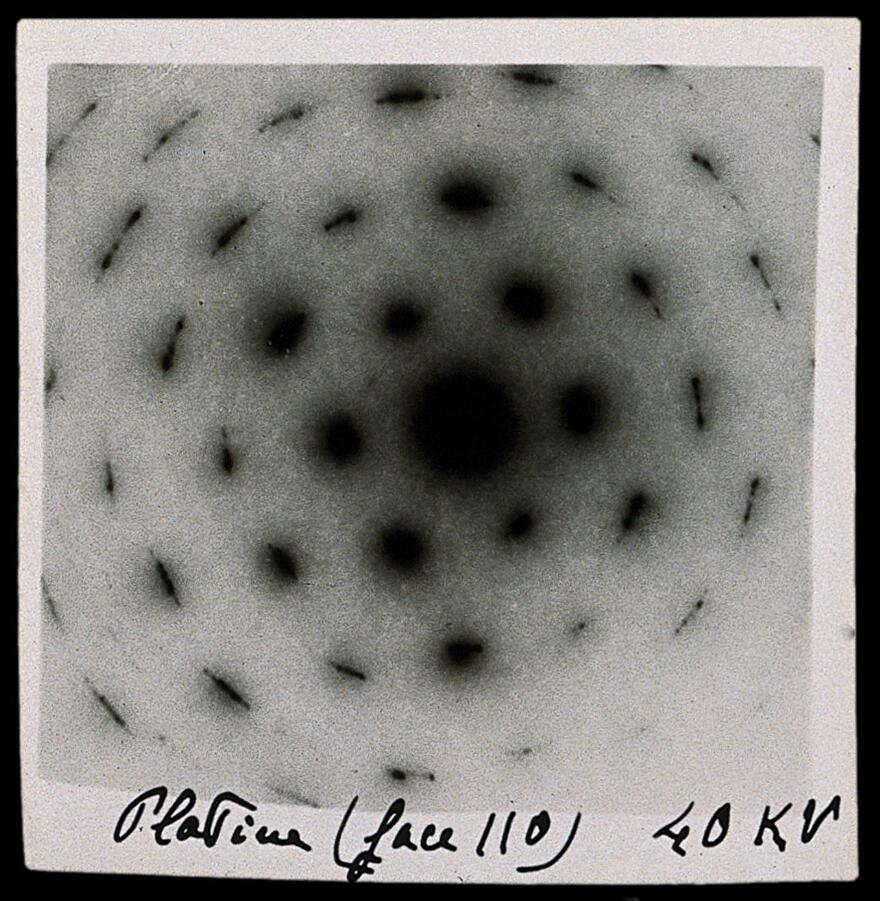
\includegraphics[height=0.80\textheight]{figures/JJTrillat_ElectronDiffractionPt.jpg}
    \end{center}
\footnotetext[1]{https://wellcomecollection.org/works/gc6a9472}
\end{frame}
}

{
\DarkMode
\begin{frame}
    \frametitle{The big picture}
    \framesubtitle{But physics is about 400 years old}

    \begin{columns}
        \begin{column}{0.5\textwidth}
        \begin{center}
            \tiny{Equations of motion}
        \end{center}
        \end{column}
        \begin{column}{0.5\textwidth}
        \begin{center}
            \tiny{Inv. square laws}
        \end{center}
        \end{column}
    \end{columns}

    \begin{columns}
        \begin{column}{0.5\textwidth}
            % planets orbiting
        \end{column}
        \begin{column}{0.5\textwidth}
            % cavendish torsion balance
        \end{column}
    \end{columns}

\begin{center}
    Fundamentals: \textbf{1600s}
\end{center}
\end{frame}
}

{
\DarkMode
\begin{frame}
    \frametitle{The big picture}
    \framesubtitle{And biology/medicine is about 200 years old}

    \begin{columns}
        \begin{column}{0.5\textwidth}
            \begin{center}
                \small{Genetics}
            \end{center}
        \end{column}
        \begin{column}{0.5\textwidth}
            \begin{center}
                \small{Cell theory}
            \end{center}
        \end{column}
    \end{columns}

    \begin{columns}
        \begin{column}{0.43\textwidth}
        % some varieties of pea
            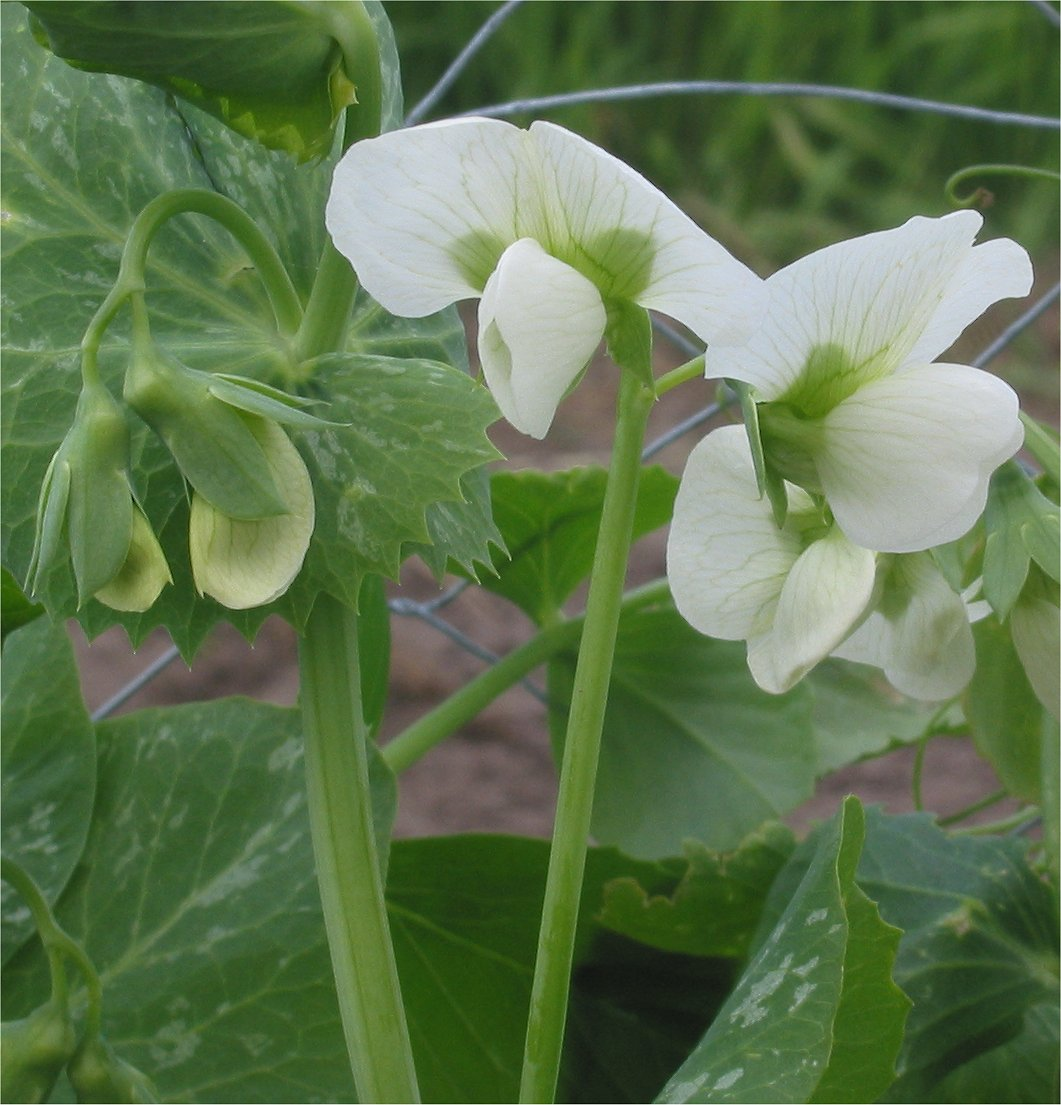
\includegraphics[width=\textwidth]{figures/Doperwt_rijserwt_bloemen_Pisum_sativum.jpg}
        \end{column}
        \begin{column}{0.57\textwidth}
            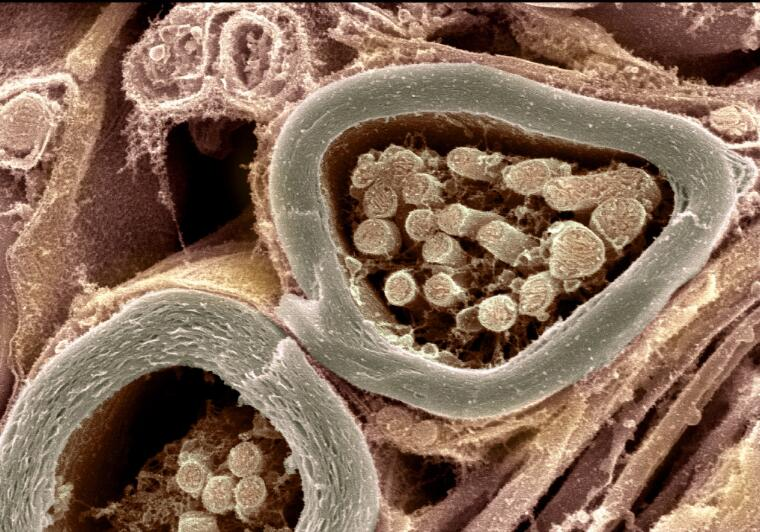
\includegraphics[width=\textwidth]{figures/myelin.jpg}
        \end{column}
    \end{columns}

\begin{center}
    Fundamentals: \textbf{1800s}
\end{center}

\footnotetext[1]{https://commons.wikimedia.org/wiki/User:Rasbak}
\footnotetext[2]{https://wellcomecollection.org/works/ugyj9njv}
\end{frame}
}

{
\DarkMode
\begin{frame}
    \setbeamercolor{item}{fg=white}
    \setbeamercolor{normal text}{fg=white}
    \usebeamercolor[fg]{normal text}
    \frametitle{The big picture}
    \framesubtitle{The value of mechanistic models}
    \begin{columns}
        \begin{column}{0.5\textwidth}
        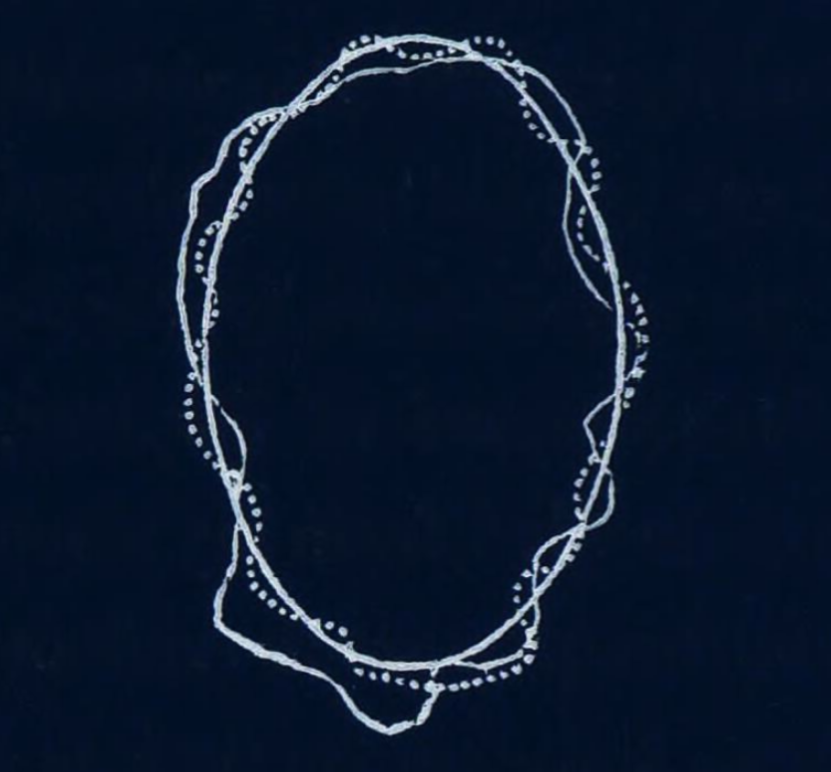
\includegraphics[width=\textwidth]{figures/Orbit2_Wellcome-inv.png}
        %\begin{center}
        %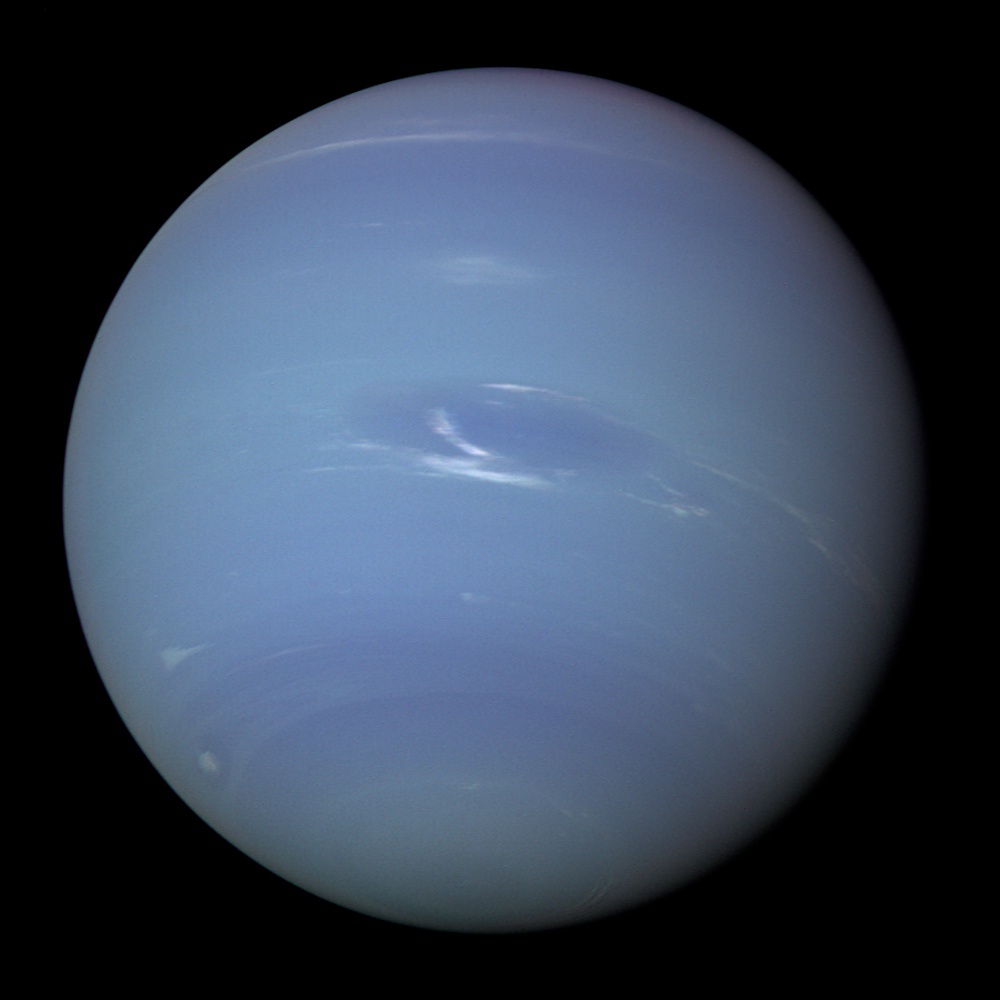
\includegraphics[width=0.65\textwidth]{figures/Neptune_-_Voyager_2_(29347980845)_flatten_crop.jpg} 
        %\end{center}

        %$\uparrow$ within $1^\circ$ of predicted location
        \end{column}
        \begin{column}{0.5\textwidth}
        \begin{itemize}
            \item Model with specific mechanism
            \item Exhausted known factors
            \item Residuals = new factor
            \item Model predicted \emph{size and location} of unknown planet
        \end{itemize}
        \end{column}
    \end{columns}
\footnotetext[1]{J.P. Nichol, ``The planet Neptune: an exposition and history''
1849}
\end{frame}
}

{
\DarkMode
\begin{frame}
    \setbeamercolor{item}{fg=white}
    \setbeamercolor{normal text}{fg=white}
    \usebeamercolor[fg]{normal text}
    \frametitle{The big picture}
    \framesubtitle{The value of mechanistic models}
    \begin{columns}
        \begin{column}{0.5\textwidth}
        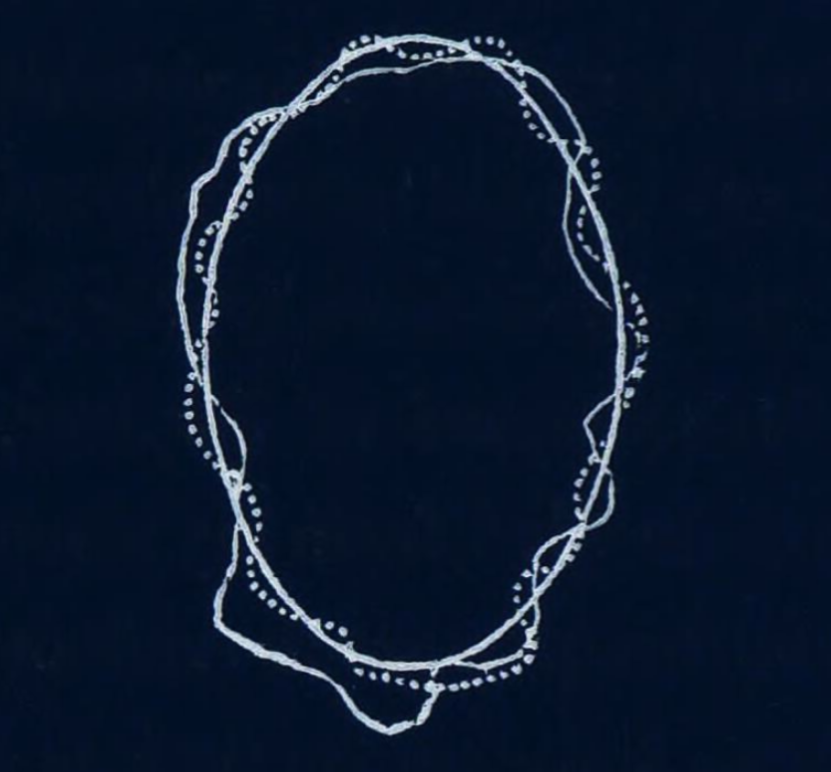
\includegraphics[width=\textwidth]{figures/Orbit2_Wellcome-inv.png}
        \end{column}
        \begin{column}{0.5\textwidth}
        \begin{center}
        \includegraphics[width=0.65\textwidth]{figures/Neptune_-_Voyager_2_(29347980845)_flatten_crop.jpg} 
        \end{center}

        $\uparrow$ within $1^\circ$ of predicted location
        \end{column}
    \end{columns}
\footnotetext[1]{J.P. Nichol, ``The planet Neptune: an exposition and history''
1849}
\end{frame}
}




% Acknowledgements

\begin{frame}
    \frametitle{Acknowledgements + collaborators}
    \framesubtitle{for their \emph{in kind} support}
    \begin{columns}
        \begin{column}{0.5\textwidth}
        \includegraphics[width=\textwidth]{figures/logo_big.jpg}
        \end{column}
        \begin{column}{0.5\textwidth}
        % Manchester NHS FT

        \end{column}
    \end{columns}
    \begin{columns}
        \begin{column}{0.5\textwidth}
        \begin{center}
        \includegraphics[width=0.4\textwidth]{figures/W-Logo_Purple1}
        \end{center}

        The University of Washington
        \end{column}
        \begin{column}{0.5\textwidth}
        In order of appearance...

        \begin{itemize}
            \item Ivana Bo\v{z}i\'{c}
            \item Hans Clevers
            \item Gareth Evans
            \item Xanthe Hoad
            \item Miriam Smith
        \end{itemize}

        \end{column}
    \end{columns}
    % UoM
    % UW
    % NHS
    % InSync (maybe)

    % Budget: £0
\end{frame}

{
\DarkMode
\setbeamertemplate{background}
{
    \includegraphics[width=1.0\paperwidth]{figures/SOLARECLIPSE2021FORDISTROHighRes.jpg}
}
\begin{frame}
    \frametitle{}

    \;

    \;

    \;

    \;

    \begin{center}
        Thank you for listening!
    \end{center}
\end{frame}
}
% I don't *need* a job
% Mostly want new collaborations especially with experimental components
% Would be nice to spend more time doing research
% Ideal: externally funded position

\end{document} 
